
%% bare_conf.tex
%% V1.4b
%% 2015/08/26
%% by Michael Shell
%% See:
%% http://www.michaelshell.org/
%% for current contact information.
%%
%% This is a skeleton file demonstrating the use of IEEEtran.cls
%% (requires IEEEtran.cls version 1.8b or later) with an IEEE
%% conference paper.
%%
%% Support sites:
%% http://www.michaelshell.org/tex/ieeetran/
%% http://www.ctan.org/pkg/ieeetran
%% and
%% http://www.ieee.org/

%%*************************************************************************
%% Legal Notice:
%% This code is offered as-is without any warranty either expressed or
%% implied; without even the implied warranty of MERCHANTABILITY or
%% FITNESS FOR A PARTICULAR PURPOSE! 
%% User assumes all risk.
%% In no event shall the IEEE or any contributor to this code be liable for
%% any damages or losses, including, but not limited to, incidental,
%% consequential, or any other damages, resulting from the use or misuse
%% of any information contained here.
%%
%% All comments are the opinions of their respective authors and are not
%% necessarily endorsed by the IEEE.
%%
%% This work is distributed under the LaTeX Project Public License (LPPL)
%% ( http://www.latex-project.org/ ) version 1.3, and may be freely used,
%% distributed and modified. A copy of the LPPL, version 1.3, is included
%% in the base LaTeX documentation of all distributions of LaTeX released
%% 2003/12/01 or later.
%% Retain all contribution notices and credits.
%% ** Modified files should be clearly indicated as such, including  **
%% ** renaming them and changing author support contact information. **
%%*************************************************************************
% *** Authors should verify (and, if needed, correct) their LaTeX system  ***
% *** with the testflow diagnostic prior to trusting their LaTeX platform ***
% *** with production work. The IEEE's font choices and paper sizes can   ***
% *** trigger bugs that do not appear when using other class files.       ***                          ***
% The testflow support page is at:
% http://www.michaelshell.org/tex/testflow/





\documentclass[conference]{IEEEtran}
\IEEEoverridecommandlockouts
% Some Computer Society conferences also require the compsoc mode option,
% but others use the standard conference format.
%
% If IEEEtran.cls has not been installed into the LaTeX system files,
% manually specify the path to it like:
% \documentclass[conference]{../sty/IEEEtran}






% Some very useful LaTeX packages include:
% (uncomment the ones you want to load)


% *** MISC UTILITY PACKAGES ***
%
%\usepackage{ifpdf}
% Heiko Oberdiek's ifpdf.sty is very useful if you need conditional
% compilation based on whether the output is pdf or dvi.
% usage:
% \ifpdf
%   % pdf code
% \else
%   % dvi code
% \fi
% The latest version of ifpdf.sty can be obtained from:
% http://www.ctan.org/pkg/ifpdf
% Also, note that IEEEtran.cls V1.7 and later provides a builtin
% \ifCLASSINFOpdf conditional that works the same way.
% When switching from latex to pdflatex and vice-versa, the compiler may
% have to be run twice to clear warning/error messages.



\usepackage{float}



% *** CITATION PACKAGES ***
%
\usepackage{cite}
% cite.sty was written by Donald Arseneau
% V1.6 and later of IEEEtran pre-defines the format of the cite.sty package
% \cite{} output to follow that of the IEEE. Loading the cite package will
% result in citation numbers being automatically sorted and properly
% "compressed/ranged". e.g., [1], [9], [2], [7], [5], [6] without using
% cite.sty will become [1], [2], [5]--[7], [9] using cite.sty. cite.sty's
% \cite will automatically add leading space, if needed. Use cite.sty's
% noadjust option (cite.sty V3.8 and later) if you want to turn this off
% such as if a citation ever needs to be enclosed in parenthesis.
% cite.sty is already installed on most LaTeX systems. Be sure and use
% version 5.0 (2009-03-20) and later if using hyperref.sty.
% The latest version can be obtained at:
% http://www.ctan.org/pkg/cite
% The documentation is contained in the cite.sty file itself.

\newtheorem{definition}{Definition}
%\usepackage{algpseudocode}


\usepackage{color}
\usepackage{gensymb}


%footnote package


%\usepackage[vlined,ruled]{algorithm2e}






% *** GRAPHICS RELATED PACKAGES ***
%
\ifCLASSINFOpdf
   \usepackage[pdftex]{graphicx}
  % declare the path(s) where your graphic files are
  % \graphicspath{{../pdf/}{../jpeg/}}
  % and their extensions so you won't have to specify these with
  % every instance of \includegraphics
  % \DeclareGraphicsExtensions{.pdf,.jpeg,.png}
\else
  % or other class option (dvipsone, dvipdf, if not using dvips). graphicx
  % will default to the driver specified in the system graphics.cfg if no
  % driver is specified.
  % \usepackage[dvips]{graphicx}
  % declare the path(s) where your graphic files are
  % \graphicspath{{../eps/}}
  % and their extensions so you won't have to specify these with
  % every instance of \includegraphics
  % \DeclareGraphicsExtensions{.eps}
\fi
% graphicx was written by David Carlisle and Sebastian Rahtz. It is
% required if you want graphics, photos, etc. graphicx.sty is already
% installed on most LaTeX systems. The latest version and documentation
% can be obtained at: 
% http://www.ctan.org/pkg/graphicx
% Another good source of documentation is "Using Imported Graphics in
% LaTeX2e" by Keith Reckdahl which can be found at:
% http://www.ctan.org/pkg/epslatex
%
% latex, and pdflatex in dvi mode, support graphics in encapsulated
% postscript (.eps) format. pdflatex in pdf mode supports graphics
% in .pdf, .jpeg, .png and .mps (metapost) formats. Users should ensure
% that all non-photo figures use a vector format (.eps, .pdf, .mps) and
% not a bitmapped formats (.jpeg, .png). The IEEE frowns on bitmapped formats
% which can result in "jaggedy"/blurry rendering of lines and letters as
% well as large increases in file sizes.
%
% You can find documentation about the pdfTeX application at:
% http://www.tug.org/applications/pdftex





% *** MATH PACKAGES ***
%
\usepackage{amsmath}
% A popular package from the American Mathematical Society that provides
% many useful and powerful commands for dealing with mathematics.
%
% Note that the amsmath package sets \interdisplaylinepenalty to 10000
% thus preventing page breaks from occurring within multiline equations. Use:
%\interdisplaylinepenalty=2500
% after loading amsmath to restore such page breaks as IEEEtran.cls normally
% does. amsmath.sty is already installed on most LaTeX systems. The latest
% version and documentation can be obtained at:
% http://www.ctan.org/pkg/amsmath





% *** SPECIALIZED LIST PACKAGES ***
%
\usepackage{algorithm, algpseudocode}
\usepackage{algorithmicx}
% algorithmic.sty was written by Peter Williams and Rogerio Brito.
% This package provides an algorithmic environment fo describing algorithms.
% You can use the algorithmic environment in-text or within a figure
% environment to provide for a floating algorithm. Do NOT use the algorithm
% floating environment provided by algorithm.sty (by the same authors) or
% algorithm2e.sty (by Christophe Fiorio) as the IEEE does not use dedicated
% algorithm float types and packages that provide these will not provide
% correct IEEE style captions. The latest version and documentation of
% algorithmic.sty can be obtained at:
% http://www.ctan.org/pkg/algorithms
% Also of interest may be the (relatively newer and more customizable)
% algorithmicx.sty package by Szasz Janos:
% http://www.ctan.org/pkg/algorithmicx

%\makeatletter
%\newcommand\fs@norules{\def\@fs@cfont{\bfseries}\let\@fs@capt\floatc@ruled
%  \def\@fs@pre{}%
%  \def\@fs@post{}%
%  \def\@fs@mid{\kern3pt}%
%  \let\@fs@iftopcapt\iftrue}
%\makeatother
%\floatstyle{norules}
%\restylefloat{algorithm}




% *** ALIGNMENT PACKAGES ***
%
%\usepackage{array}
% Frank Mittelbach's and David Carlisle's array.sty patches and improves
% the standard LaTeX2e array and tabular environments to provide better
% appearance and additional user controls. As the default LaTeX2e table
% generation code is lacking to the point of almost being broken with
% respect to the quality of the end results, all users are strongly
% advised to use an enhanced (at the very least that provided by array.sty)
% set of table tools. array.sty is already installed on most systems. The
% latest version and documentation can be obtained at:
% http://www.ctan.org/pkg/array


% IEEEtran contains the IEEEeqnarray family of commands that can be used to
% generate multiline equations as well as matrices, tables, etc., of high
% quality.
\usepackage{caption}

\captionsetup[algorithm]{labelsep=colon}


% *** SUBFIGURE PACKAGES ***
%\ifCLASSOPTIONcompsoc
%  \usepackage[caption=false,font=normalsize,labelfont=sf,textfont=sf]{subfig}
%\else
%  \usepackage[caption=false,font=footnotesize]{subfig}
%\fi
% subfig.sty, written by Steven Douglas Cochran, is the modern replacement
% for subfigure.sty, the latter of which is no longer maintained and is
% incompatible with some LaTeX packages including fixltx2e. However,
% subfig.sty requires and automatically loads Axel Sommerfeldt's caption.sty
% which will override IEEEtran.cls' handling of captions and this will result
% in non-IEEE style figure/table captions. To prevent this problem, be sure
% and invoke subfig.sty's "caption=false" package option (available since
% subfig.sty version 1.3, 2005/06/28) as this is will preserve IEEEtran.cls
% handling of captions.
% Note that the Computer Society format requires a larger sans serif font
% than the serif footnote size font used in traditional IEEE formatting
% and thus the need to invoke different subfig.sty package options depending
% on whether compsoc mode has been enabled.
%
% The latest version and documentation of subfig.sty can be obtained at:
% http://www.ctan.org/pkg/subfig




 
 \usepackage[bottom]{footmisc}

% *** FLOAT PACKAGES ***
%
%\usepackage{fixltx2e}


% fixltx2e, the successor to the earlier fix2col.sty, was written by
% Frank Mittelbach and David Carlisle. This package corrects a few problems
% in the LaTeX2e kernel, the most notable of which is that in current
% LaTeX2e releases, the ordering of single and double column floats is not
% guaranteed to be preserved. Thus, an unpatched LaTeX2e can allow a
% single column figure to be placed prior to an earlier double column
% figure.
% Be aware that LaTeX2e kernels dated 2015 and later have fixltx2e.sty's
% corrections already built into the system in which case a warning will
% be issued if an attempt is made to load fixltx2e.sty as it is no longer
% needed.
% The latest version and documentation can be found at:
% http://www.ctan.org/pkg/fixltx2e


%\usepackage{stfloats}
% stfloats.sty was written by Sigitas Tolusis. This package gives LaTeX2e
% the ability to do double column floats at the bottom of the page as well
% as the top. (e.g., "\begin{figure*}[!b]" is not normally possible in
% LaTeX2e). It also provides a command:
%\fnbelowfloat
% to enable the placement of footnotes below bottom floats (the standard
% LaTeX2e kernel puts them above bottom floats). This is an invasive package
% which rewrites many portions of the LaTeX2e float routines. It may not work
% with other packages that modify the LaTeX2e float routines. The latest
% version and documentation can be obtained at:
% http://www.ctan.org/pkg/stfloats
% Do not use the stfloats baselinefloat ability as the IEEE does not allow
% \baselineskip to stretch. Authors submitting work to the IEEE should note
% that the IEEE rarely uses double column equations and that authors should try
% to avoid such use. Do not be tempted to use the cuted.sty or midfloat.sty
% packages (also by Sigitas Tolusis) as the IEEE does not format its papers in
% such ways.
% Do not attempt to use stfloats with fixltx2e as they are incompatible.
% Instead, use Morten Hogholm'a dblfloatfix which combines the features
% of both fixltx2e and stfloats:
%
% \usepackage{dblfloatfix}
% The latest version can be found at:
% http://www.ctan.org/pkg/dblfloatfix




% *** PDF, URL AND HYPERLINK PACKAGES ***
%
\usepackage{url}
% url.sty was written by Donald Arseneau. It provides better support for
% handling and breaking URLs. url.sty is already installed on most LaTeX
% systems. The latest version and documentation can be obtained at:
% http://www.ctan.org/pkg/url
% Basically, \url{my_url_here}.




% *** Do not adjust lengths that control margins, column widths, etc. ***
% *** Do not use packages that alter fonts (such as pslatex).         ***
% There should be no need to do such things with IEEEtran.cls V1.6 and later.
% (Unless specifically asked to do so by the journal or conference you plan
% to submit to, of course. )


% correct bad hyphenation here
%\hyphenation{op-tical net-works semi-conduc-tor}


\begin{document}
%
% paper title
% Titles are generally capitalized except for words such as a, an, and, as,
% at, but, by, for, in, nor, of, on, or, the, to and up, which are usually
% not capitalized unless they are the first or last word of the title.
% Linebreaks \\ can be used within to get better formatting as desired.
% Do not put math or special symbols in the title.
%\title{Towards a Provenance-Aware Internet of Things (IoT) System}

%\title{IoT Device Sensor Data Anomaly-based Intrusion Detection using Provenance Graphs}
\title{Anomaly-based Intrusion Detection of IoT Device Sensor Data using Provenance Graphs\\
{\footnotesize \textsuperscript{}}
\thanks{This material is based upon work supported by the National Science Foundation
under Grant No. CNS-1646317 and the U.S. Department of Homeland Security under
Grant Award Number 2017-ST-062-000003. Any opinions, findings, and conclusions
or recommendations expressed in this material are those of the authors and do
not necessarily reflect the views of the National Science Foundation and
should not be interpreted as necessarily representing the official policies,
either expressed or implied, of the U.S. Department of Homeland Security.}
}


%A provenance-graph based approach to anomaly-based intrusion detection of sensor data in IoT Devices

%\title{Provenance Graph Based Sensor Data Anomaly Detection in IoT Devices }


% author names and affiliations
% use a multiple column layout for up to three different
% affiliations

%\author{\IEEEauthorblockN{Michael Shell}
%\IEEEauthorblockA{School of Electrical and\\Computer Engineering\\
%Georgia Institute of Technology\\
%Atlanta, Georgia 30332--0250\\
%Email: http://www.michaelshell.org/contact.html}
%\and
%\IEEEauthorblockN{Homer Simpson}
%\IEEEauthorblockA{Twentieth Century Fox\\
%Springfield, USA\\
%Email: homer@thesimpsons.com}
%\and
%\IEEEauthorblockN{James Kirk\\ and Montgomery Scott}
%\IEEEauthorblockA{Starfleet Academy\\
%San Francisco, California 96678--2391\\
%Telephone: (800) 555--1212\\
%Fax: (888) 555--1212}}

% conference papers do not typically use \thanks and this command
% is locked out in conference mode. If really needed, such as for
% the acknowledgment of grants, issue a \IEEEoverridecommandlockouts
% after \documentclass

% for over three affiliations, or if they all won't fit within the width
% of the page, use this alternative format:
% 
\author{\IEEEauthorblockN{
Ebelechukwu Nwafor, Andre Campbell and
Gedare Bloom}
\IEEEauthorblockA{Department of Electrical Engineering and Computer Science\\
Howard University,
Washington, DC 20059\\ Email: ebelechukwu.nwafor@bison.howard.edu}
%\IEEEauthorblockA{\IEEEauthorrefmark{2}Twentieth Century Fox, Springfield, USA\\
%Email: homer@thesimpsons.com}
%\IEEEauthorblockA{\IEEEauthorrefmark{3}Starfleet Academy, San Francisco, California 96678-2391\\
%Telephone: (800) 555--1212, Fax: (888) 555--1212}
%\IEEEauthorblockA{\IEEEauthorrefmark{4}Tyrell Inc., 123 Replicant Street, Los Angeles, California 90210--4321}
}




%\author{\IEEEauthorblockN{Ebelechukwu Nwafor\IEEEauthorrefmark{1},
%Gedare Bloom\IEEEauthorrefmark{2}, Andre Campbell\IEEEauthorrefmark{3} and
%David Hill\IEEEauthorrefmark{4}}
%\IEEEauthorblockA{Department of Electrical Engineering and Computer Science\\
%\\ 2366 Sixth Street, NW, Washington, DC 20059\\
%Email: \IEEEauthorrefmark{1}ebelechukwu.nwafor@bison.howard.edu,
%\IEEEauthorrefmark{2}gedare@scs.howard.edu,
%\IEEEauthorrefmark{3}author.three@add.on.net,
%\IEEEauthorrefmark{4}author.four@add.on.net}}


% use for special paper notices
%\IEEEspecialpapernotice{(Invited Paper)}




% make the title area
\maketitle

% As a general rule, do not put math, special symbols or citations
% in the abstract
\begin{abstract}
The Internet of Things (IoT) has revolutionized the way humans interact with devices. Unfortunately, this technological revolution has been met with privacy and security challenges. One major concern is the notion of malicious intrusions. A common way of detecting a malicious intrusion is by treating an attack as an  anomaly and using anomaly detection techniques to detect the source of intrusion. In a given IoT device, provenance, which denotes causality between system events, offers immense benefit for intrusion detection. Provenance provides a comprehensive history of activity performed on a system's data, which indirectly ensures device trust. In this paper, we propose an approach to intrusion detection of IoT devices that leverages sensor data flow as seen through provenance graphs. In this approach, an observed provenance graph is compared to an application's known provenance graph. This comparison involves the dimensionality reduction of a provenance graph to a vector space representation and similarity metric. We evaluated our approach on an IoT application which simulates a climate control system. 

%of our approach by comparing provenance graphs generated from sample IoT applications and determine the number of false positive, true positive and false negative rates.

%We compare our method to two known anomaly detection algorithms. 
\end{abstract}

\begin{IEEEkeywords}Anomaly detection, Intrusion detection, Internet of Things, Data Provenance

\end{IEEEkeywords}

\section{Introduction}

Over the years, IoT devices have become an essential part of our daily lives in commercial, industrial, and infrastructure systems. These devices offer immense benefits to consumers by interacting with our physical environment through sensors and actuators which allows device automation thereby improving efficiency. Unfortunately, the proliferation of IoT devices has led to an increase in the number of remotely exploitable vulnerabilities leading to new attack vectors that could have disastrous financial and physical implications \cite{barcena2015insecurity}. In 2015, security researchers demonstrated a vulnerability on the Jeep vehicle which allowed remote control of the digital system over the Internet \cite{jeep_vulnerabilty}. In 2016, researchers discovered a vulnerability that allows internet connected smart thermostats be subject to remote ransomware attacks in which an attacker gains sole control of the thermostat until a fee is paid \cite{smart_thermostat}. These are a few example of some of the potential malicious vulnerabilities that could have devastating long lasting impact on an IoT system. \par Intrusion detection \cite{Lazarevic2005} is the process of discovering malicious exploits that exist in a system (i.e. network, host). One way of detecting an intrusion is by the use of anomaly detection techniques. An anomaly, also referred to as an outlier, is defined as data that deviates from the normal system behavior. This could be indicative of a system fault or that a system has been compromised by a malicious event. Due to the sensitive nature of safety critical systems, detecting current and future malicious attacks is of utmost importance.

 
%\par Sensors and actuators are important components of an IoT device. Sensors detects environmental signals which are relayed as electric or optical output. An actuator on the other hand, performs task specified by a control signal (e.g sensor's signal or manual input). From pacemakers to motor vehicles, IoT devices generate an unprecedented amount  of sensor data, it is important to track the information flow of sensor based events in order to uncover anomalous relationships that exists between sensor based events in an IoT device. In this paper, we motivate the need for IoT device anomaly detection.



 \par Unlike most host-based intrusion detection system which utilize system call frequencies to determine anomalous system events, our approach detects anomalies by leveraging the information flow of sensor events as represented in a provenance graph. Provenance graph captures a comprehensive history of transformations that occurs on a data object during its lifecycle. It offers a way of representing relationships that exist between multiple data objects. This, in turn, can be used to detect system faults or anomalous system events such as malicious intrusions. We propose an approach to identifying anomalous sensor events using provenance graphs. This approach involves the use of a similarity measure to compare observed provenance graphs with provenance graph derived from an application's normal execution. The result of the algorithm generates an anomaly score in which a threshold is set that classifies an observed provenance graph as either anomalous or benign. We evaluate the effectiveness of our approach with a sample IoT application which simulates a climate control system by comparing the false positive, false negative and true positive rate.




%\par In summary, our technical contributions are outlined in detail as follows:
%
%
%%Anomaly detection has applications in domains such as intrusion detection, fraud detection, medical health devices, sensor fault detection, and web spam.
%
%
%
%%We also propose a hybrid classification algorithm based on $k$- Nearest Neighbors ($k$-NN), and $k$ means clustering. Anomalous events are detected based on their proximity to known normal provenance graph. Our technical contributions are outlined in detail as follows:
%
%\begin{itemize}[]
%
%\item We introduce an anomaly detection algorithm for detecting malicious intrusions in an IoT device using provenance graphs. 
%
%%\item We take a hybrid approach to anomaly detection by combining clustering, classification, and density-based techniques. In the training phase, the unlabeled data set is clustered into two groups (where $k \lesssim 2$). The density of each cluster is observed using the Local Outlier Factor (LOF) to determine which cluster is considered the normal or an anomaly. In the test phase,  $k$ nearest neighbor algorithm is used to classify incoming data instances as normal or anomaly.
%
%%\item We propose two anomaly detection techniques for IoT devices using provenance graphs. The first algorithm is based on the similarity between provenance graphs in the learning and detection phases which is achieved by using a similarity metric. The second algorithm is a hybrid approach which uses clustering algorithm, DBSCAN, and $k$-nearest neighbor algorithm.
%
%
%
%\item We evaluate the effectiveness of our approach to anomaly detection with a dataset from an IoT application by comparing the false positive, false negative and true positive rate of our proposed approach. Detailed results are presented in sections V. 
%
%\end{itemize}

The remaining portion of this paper is organized as follows. In section 2, we discuss background information on anomaly detection and provenance graphs. In section 3, we describe our threat model and assumptions, In section 4, we discuss details of our graph based anomaly detection algorithm. In section 5, we describes our experimental design and evaluation. In section 6 we describe related work on intrusion detection and graph based anomaly detection. Finally, in section 7, we summarize and conclude our findings.



%Graph based anomaly detection has been explored in various research.Most of the prior work focuses on static graphs using community outliers, and finding similarities from frequent substructures. 

%There are two major approach to intrusion detection. Signature based Intrusion detection and anomaly based detection.

%In recent years,the Internet of Things (IoT) has gathered significant traction which has led
%to the exponential increase in the number of devices connected to the internet. %IoT involves the connection of heterogeneous devices with sensing and actuating capabilities over the internet. 
%It has revolutionized devices to device communication, which in turn optimizes efficiency and improves the standard of living. According to a report released by Cisco, it is estimated that a total of 50 million devices will be connected to the internet by the year 2020.  With the vast amounts of connected heterogeneous devices, security and privacy risks are increased. Data provenance is instrumental to the security IoT data. Provenance describes a holistic history of operations  performed on a data object from its point of creation. Provenance can be used as a measure to ensure trust and also for forensic analysis in an event of malicious attack. Provenance collection system is of immense benefit to IoT devices however provenance incurs additional storage overhead. Continuous provenance collection has the tendency to generate more data than the data it describes. Work done by Brian et al demonstrates that changes to a source file in the Linux kernel results to two kilobytes of additional provenance data when the kernel is recompiled. Additionally, Figure x displays a graph of the growth of provenance data for a raspberry pi collecting temperature and humidity readings. This sensor reading is stored in CTF format. From the diagram we can see that the data grows rapidly with time. This motivates the need for an efficient pruning technique to reduce storage overhead that might be incurred by including provenance in an IoT application. It is of utmost importance to provide a method of pruning provenance data generated thereby reducing the storage overhead. This requirement is further motivated by the constrained memory and computing power of IoT devices. Pruning can be described as removing provenance data in order to conserve storage. 
% \par In this paper, we propose a fine-grained, policy model for provenance pruning. This model provides an expressive policy language which allows device administrators the flexibility of specifying what provenance data to store.  We argue that policy is an effective way of addressing the data pruning problem created by automatic provenance collection. With access control, we allow the flexibility of deciding what provenance data is discarded thereby eliminating unwanted provenance information. Provenance sometimes generates information that might be considered uninteresting. For example, a system collecting the provenance of system events such as device internal system state might be considered uninteresting to a researcher working on collecting temperature and humidity readings or a device administrator interested on. We implement a proof of concept system using XACML, a fine-grained attribute based access control policy language which evaluates request based on a policy specifications. XACML serves as the foundation for our framework.We compared our performance of the proposed framework with state of the art on provenance pruning (e.g web compression + dictionary). 







%IoT trace is derived in the form of CTF output. This output stream is pruned to reduce storage overhead.
%
%CTF is a binary format that allows dynamic instrumentation trace of a applications written in C/C++. The source code for applications  is compiled with the generated c code that barectf creates for the IoT trace event. 
%
%barectf is chosen for tracing IoT device because it generates ANCI C code which is lightweight and can fit into most microcontrollers.

%This mode can also the further applied for access control on resources in an IoT.
%
%Sensor based access control model for authentication and enforcement of provenance data.


%The \textit{proceedings} are the records of a conference\footnote{This
%  is a footnote}.  ACM seeks
%to give these conference by-products a uniform, high-quality
%appearance.  To do this, ACM has some rigid requirements for the
%format of the proceedings documents: there is a specified format
%(balanced double columns), a specified set of fonts (Arial or
%Helvetica and Times Roman) in certain specified sizes, a specified
%live area, centered on the page, specified size of margins, specified
%column width and gutter size.

%\section{Problem Statement}
%
%Given a set of provenance graphs, P = $\{p_1, p_2,...p_n\}$ containing provenance data from both the learning and detection phase, we want detect anomalies that might exist in P.  This involves converting elements in $P$ into a feature vector space. Anomalies are detected by comparing the similarity of graphs contained in $P$ using a similarity metric and also by using a hybrid approach as discussed in section IV


% Anomalies are detected using a hybrid approach which is a combination of clustering and classification algorithms discussed in section IV

\section{BACKGROUND}

%This section describes key concepts of Anomaly detection techniques, Provenance graphs, text-based query ranking and $k$-NN. 

\subsection{Anomaly Detection}

The notion of what constitutes an anomaly is often domain specific. Hawkins defines an anomaly as an ``observation which deviates so much from the other observations as to arouse that it was generated by a different mechanism" \cite{hawkins}. In computing, an anomaly often indicates the presence of a malicious intrusion or a system fault. For example, an anomaly could be a sudden increase in web traffic of a web server which could be indicative of a denial of service attack. Additionally, in a critical care health device such as a pacemaker, an anomalous event could be detrimental to the health of a patient which could result in the loss of life. 

%Anomaly detection consists of two phase, learning phase also known as the training phase and the test also known as the detection phase. In the training phase, the system collects training dataset. This data is considered to be a representation of the system's normal daily activity and free from malicious events. Once training dataset has been collected, the system's activities are further observed. This part is known as the testing phase. In the testing phase,  observed system behavior is compared to the learning phase to determine is an anomaly exists between the two. A threshold as defined by domain experts is used to determine if the observed data is considered an anomaly.

%Data labels are grouped into three major categories. Supervised anomaly detection, semi-supervised anomaly detection, and unsupervised anomaly detection. In supervised anomaly detection approach, training data contains instances of normal and anomalous data. Incoming data is classified based on the training data category. In semi-supervised approach, only one class of training data is collected, normal data. Incoming data that does not fit the normal class as specified by a threshold is regarded as an anomalous. In the training phase, most anomaly detection techniques use data derived from the normal system behavior.  This is referred to as one class classification. In unsupervised approach, there are no training dataset. it is believed that normal data is clustered around each and occurs more frequently than an anomaly. This is a widely used form of anomaly detection since training data which is hard to get is not requited. 


Anomaly detection involves the use of rule-based, statistical, clustering or classification techniques to determine normal or anomalous data instances. The process of determining all anomalous instances in a given dataset or system is a complex task. A major challenge in anomaly detection is providing the right feature set from the data to use for detection. Another challenge exists in defining what constitutes as normal system behavior. Most anomaly detection using point based data often fail to include the dependencies that exist between data points. 




%Graphs offers a means of modeling complex structures such as social networks, computer networks, biological DNA sequences.  




%Details on anomaly detection techniques are outlined below
%
%
%\begin{enumerate}[]
%
%
%\item Statistical-based approach: This approach involves the use of parametric or non parametric statistical inference to develop models which are used to determine if a dataset fits a statistical model. Instances that do not fit the defined statistical model are classified as an anomaly. 
%
%\item Classification: The main idea in this approach involves building models which use training data set with predefined labels (i.e normal, anomalous) to classify incoming data. Classification works in two phase: training phase and observation phase. In the training phase, data is collected which contains labels of normal and anomalous system behavior. If the dataset only contains a label of either anomalous or normal behavior, this is considered as a one class classifier. In the observation phase, incoming data is classified by defined data labels.
%\begin{itemize}
%
%\item Nearest-Neighbor: It is based on the assumption that normal data occurs in dense neighborhoods and abnormal data in sparse neighborhoods. The main idea is to assign an incoming observation data to a class based on its proximity to the closest data point in the training data set. A distance or similarity measure is used to quantify the distance between points in a dataset.  A popular form of nearest neighbor technique is the $k$-nearest neighbor which groups incoming data based on proximity to $k$ closest data point. Details on $k$- nearest neighbors is discussed in section 3.5. 
%
%\end{itemize}
%
%\item Clustering: The main idea is to group similar data instances into clusters. There are various approach to clustering. One approach looks at the density of the clusters, normal data belongs to large dense clusters while abnormal data belongs to small clusters. Another approach as treats clustering as one class which assumes that normal belongs to a cluster and abnormal data does not. Another approach looks at the distance of the data to the centroid. Centroids are seen as the center of the cluster. Normal data are  considered to be closer to the centroid than anomalies lie.
%
%\begin{itemize}
%
%\item Density: This approach is used to estimate the density of  $k$ nearest neighbors. A data instance in a dense neighborhood is considered normal while data instances in neighborhoods with a sparse density are considered anomalous. The distance from a data instance to a nearest neighbor is seen as the inverse of the density of data instances.  This approach faces an issue in which the density approach performs poorly in regions of varying densities. Local outlier factor addresses this issue. Local outlier factor is a measure of the degree of Outlieriness of each data instance contained in a data set. It is achieved by comparing the ratio of local density of k nearest neighbors to the density of a data instance. Data instances with lower density are considered outliers.
%
%\end{itemize}
%
%
%
%
%
%
%\end{enumerate}    




\subsection{Provenance Graphs}

Provenance denotes the origin of an object and all activities that occurred on it. An example of provenance can be seen with a college transcript. A transcript is the provenance of a college degree because it outlines all of the courses satisfied in order to attain a degree. In computing, data provenance, also known as data lineage, can be defined
as the history of all activities performed on a data object from its creation to its current state. Provenance ensures data trust \cite{Bertino2015}. It establishes causality between entities contained in a data object through information flow tracking thereby it allows for the verification of a data source. Provenance is represented by a directed acyclic graph (DAG) in which vertices represent various data entities and the edges correspond to the interaction between them. 

%\begin{figure}[h!]
%\begin{center}
%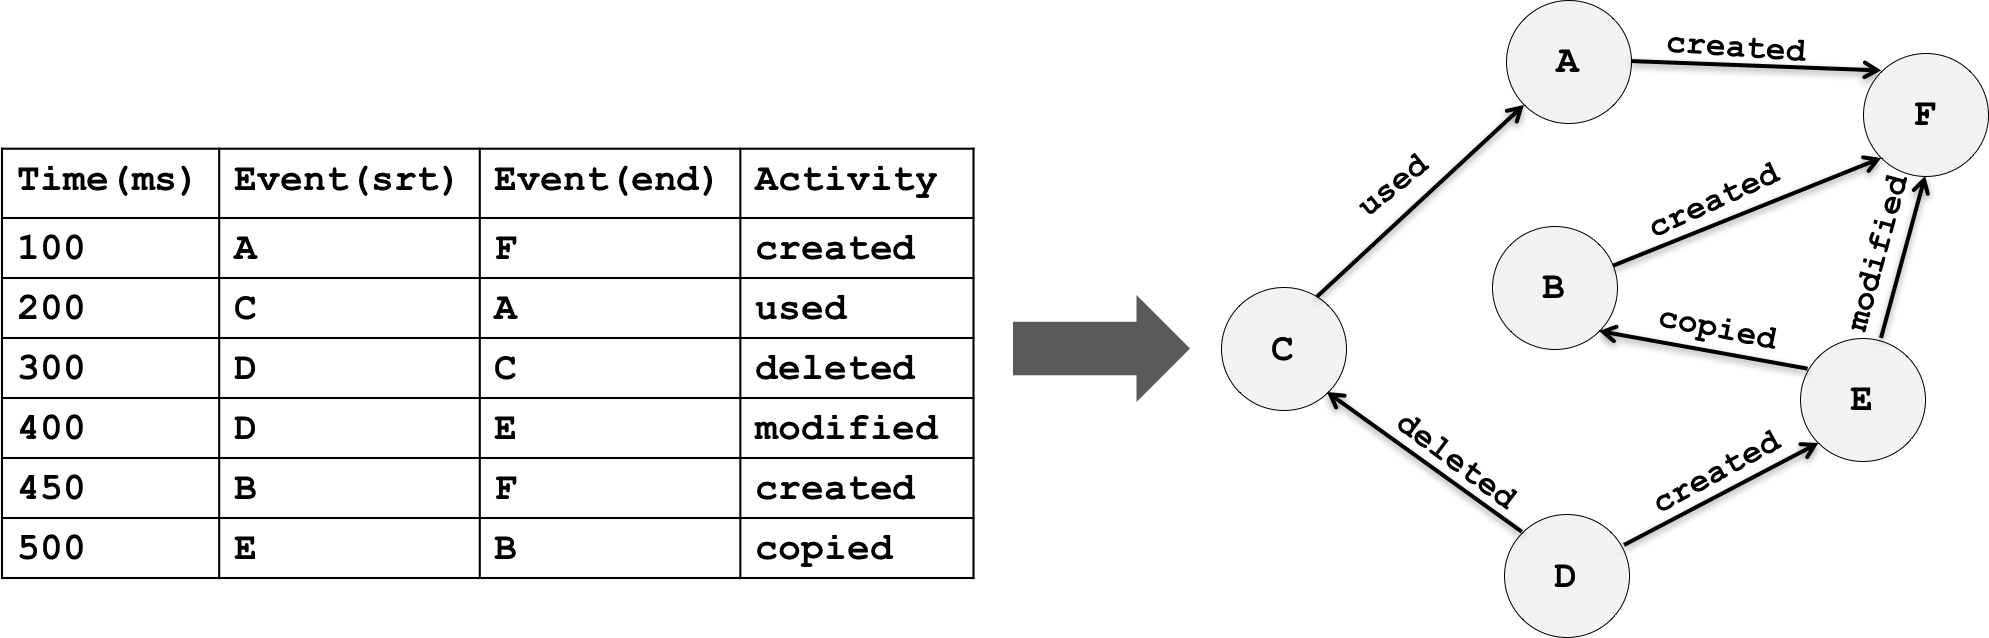
\includegraphics[height=1.4in, width=3.5in]{provenance_graph_2.png}
%\end{center}
%\caption{Provenance data transcribed to Provenance graph which depicts causal dependency between system events. The nodes represents events while the edges represents activities}
%\label{Provenance_graph}
%\end{figure}


Most provenance collection frameworks developed to track provenance use system level event sequence in an operating system \cite{pasquier-socc2017,acsac,Muniswamy-Reddy}. For most IoT device, containing limited or no operating system functionality, it is essential to use a provenance collection framework that places less emphasis on an operating system and more emphasis on application level information flow tracking. For our provenance graph generation, we use PAIoT \cite{paiot}, a provenance collection framework which tracks the information flow of sensor based event in an IoT device over its lifecycle. 


%\subsubsection{Provenance-Sensor Model}
%
%Trace data is mapped into a provenance graph representation by using the provenance-sensor model as defined in \cite{}. Provenance-sensor model denotes the information flow of sensor events leading to a decision point using provenance based ontology. Provenance-Sensor model consists of three major component: Agents, activity, and entities. We outline the components of the provenance-sensor model as follows:  

%A sensor trace is represented as a tuple $(t, e, a, s_1, r_1)$ where t is a timestamp, $e$ denotes an event, $a$ denotes an activity, $s_1$ denotes a sensor identifier and $r_1$ denotes a device identifier. There are a total of 7 edge labels between nodes in a provenance graph. These edges denote derivation, attribution, association, and generation relations.



%% 
%An event is the data that was produced by an activity.
%
%two vertices are equal if they have the same type and the same value...go to say they are no two events that are equal, events are distinct.
%
%Enitites are outputs to activities. An agent is 
%
%Get to the point of stating that a provenance graph is a set of vertices and edges and the vertices are of the three types, agent, entity, and activty
%
%
%
%Think about the vertices as abstract node, a field of nodes. A set of vertices that have the type agent, entity, and activity. The node value of a vertex includes a type. Depending on what type of node it is, it can have additional information in it.
%
%A directed graph is a set of vertices and edges, those vertices can be differentiated by their values. We make the distinction based the type and value in them. Where V is a set of vertices where each vertex has a type. The type can be one of three things, agent, entity, and activity and also a value. An agent value, is an identifier, entity's value is an event and an activity is an action. 






%\begin{figure}[h!]
%\begin{center}
%\includegraphics[height=2in, width=3.5in]{picture1.png}
%\end{center}
%\caption{Components of a provenance graph}
%\label{Provenance_Sensor}
%\end{figure}

\begin{figure}[h!]
\begin{center}
%\includegraphics[width=\columnwidth]{picture11.pdf}
%\includegraphics[width=\columnwidth]{picture12.pdf}
\includegraphics[width=\columnwidth]{picture13.pdf}
\end{center}
\caption{Components of a provenance graph where nodes represents types (agent, activity, and entity) and edges represents relationship between types}
\label{Provenance_Sensor}
\end{figure}


We formally define a provenance graph as follows:

\begin{definition}

A provenance graph is a directed acyclic graph, $p = (v_i, e_i)$ where $V$ is a set of vertices $V =\{v_1,...,v_n\}$ such that $v_i = (type, value)$. Two vertices $v_x$, $v_y$ are similar (denoted $ v_x \sim v_y$) if $v_x.type = v_y.type$ and $v_x.value = v_y. value$. $V$ consists of the following types: Agent, Entity, and Activity.  An agent is an actor that is represented by an identifier (e.g. sensor or device name). An entity is an event, which represents data that is produced as a result of an activity. An event is data that is produced as a result of an activity. An activity is an action performed by an agent or entity (e.g. read, update, create, delete). $E$ is a set of edges $E =\{e_1,..., e_n\}$ where $e_i = (v_s, v_d, label)$ and $v_s, v_d$ are source and destination vertices. $label$ takes on one of the following values: \textit{wasGeneratedBy}, \textit{used}, \textit{wasInformedBy}, \textit{wasDerivedFrom}, \textit{wasAttributedTo}, \textit{wasAssociatedWith}, \textit{actedOnBehalfOf}. 

% A decision point is a logical component of a provenance graph which denotes the evaluation of an action performed on an entity. 



\end{definition}


\begin{figure*}
\begin{center}
%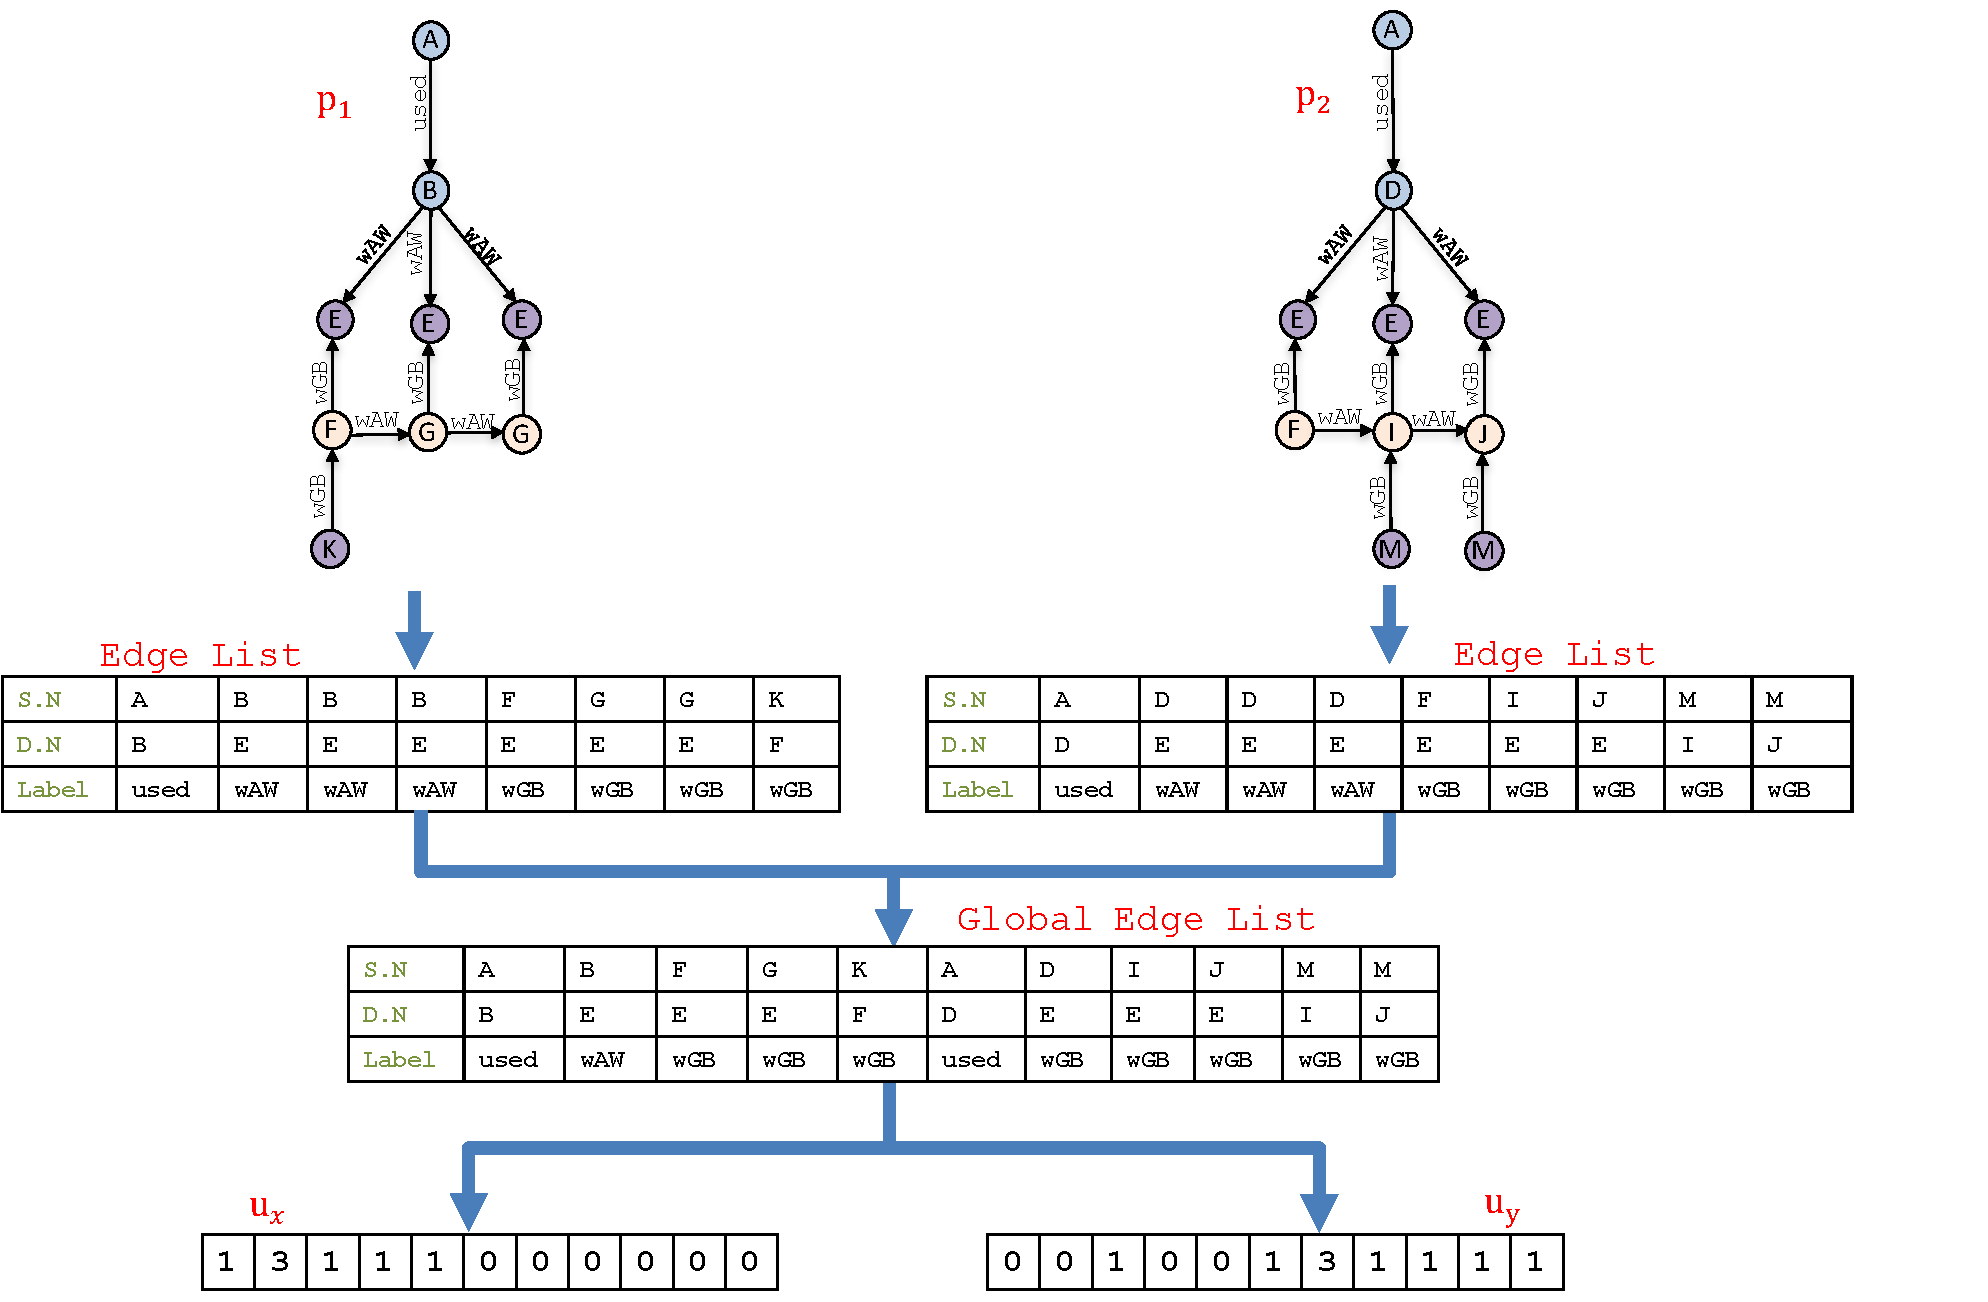
\includegraphics[width=\textwidth]{vector3.pdf}
%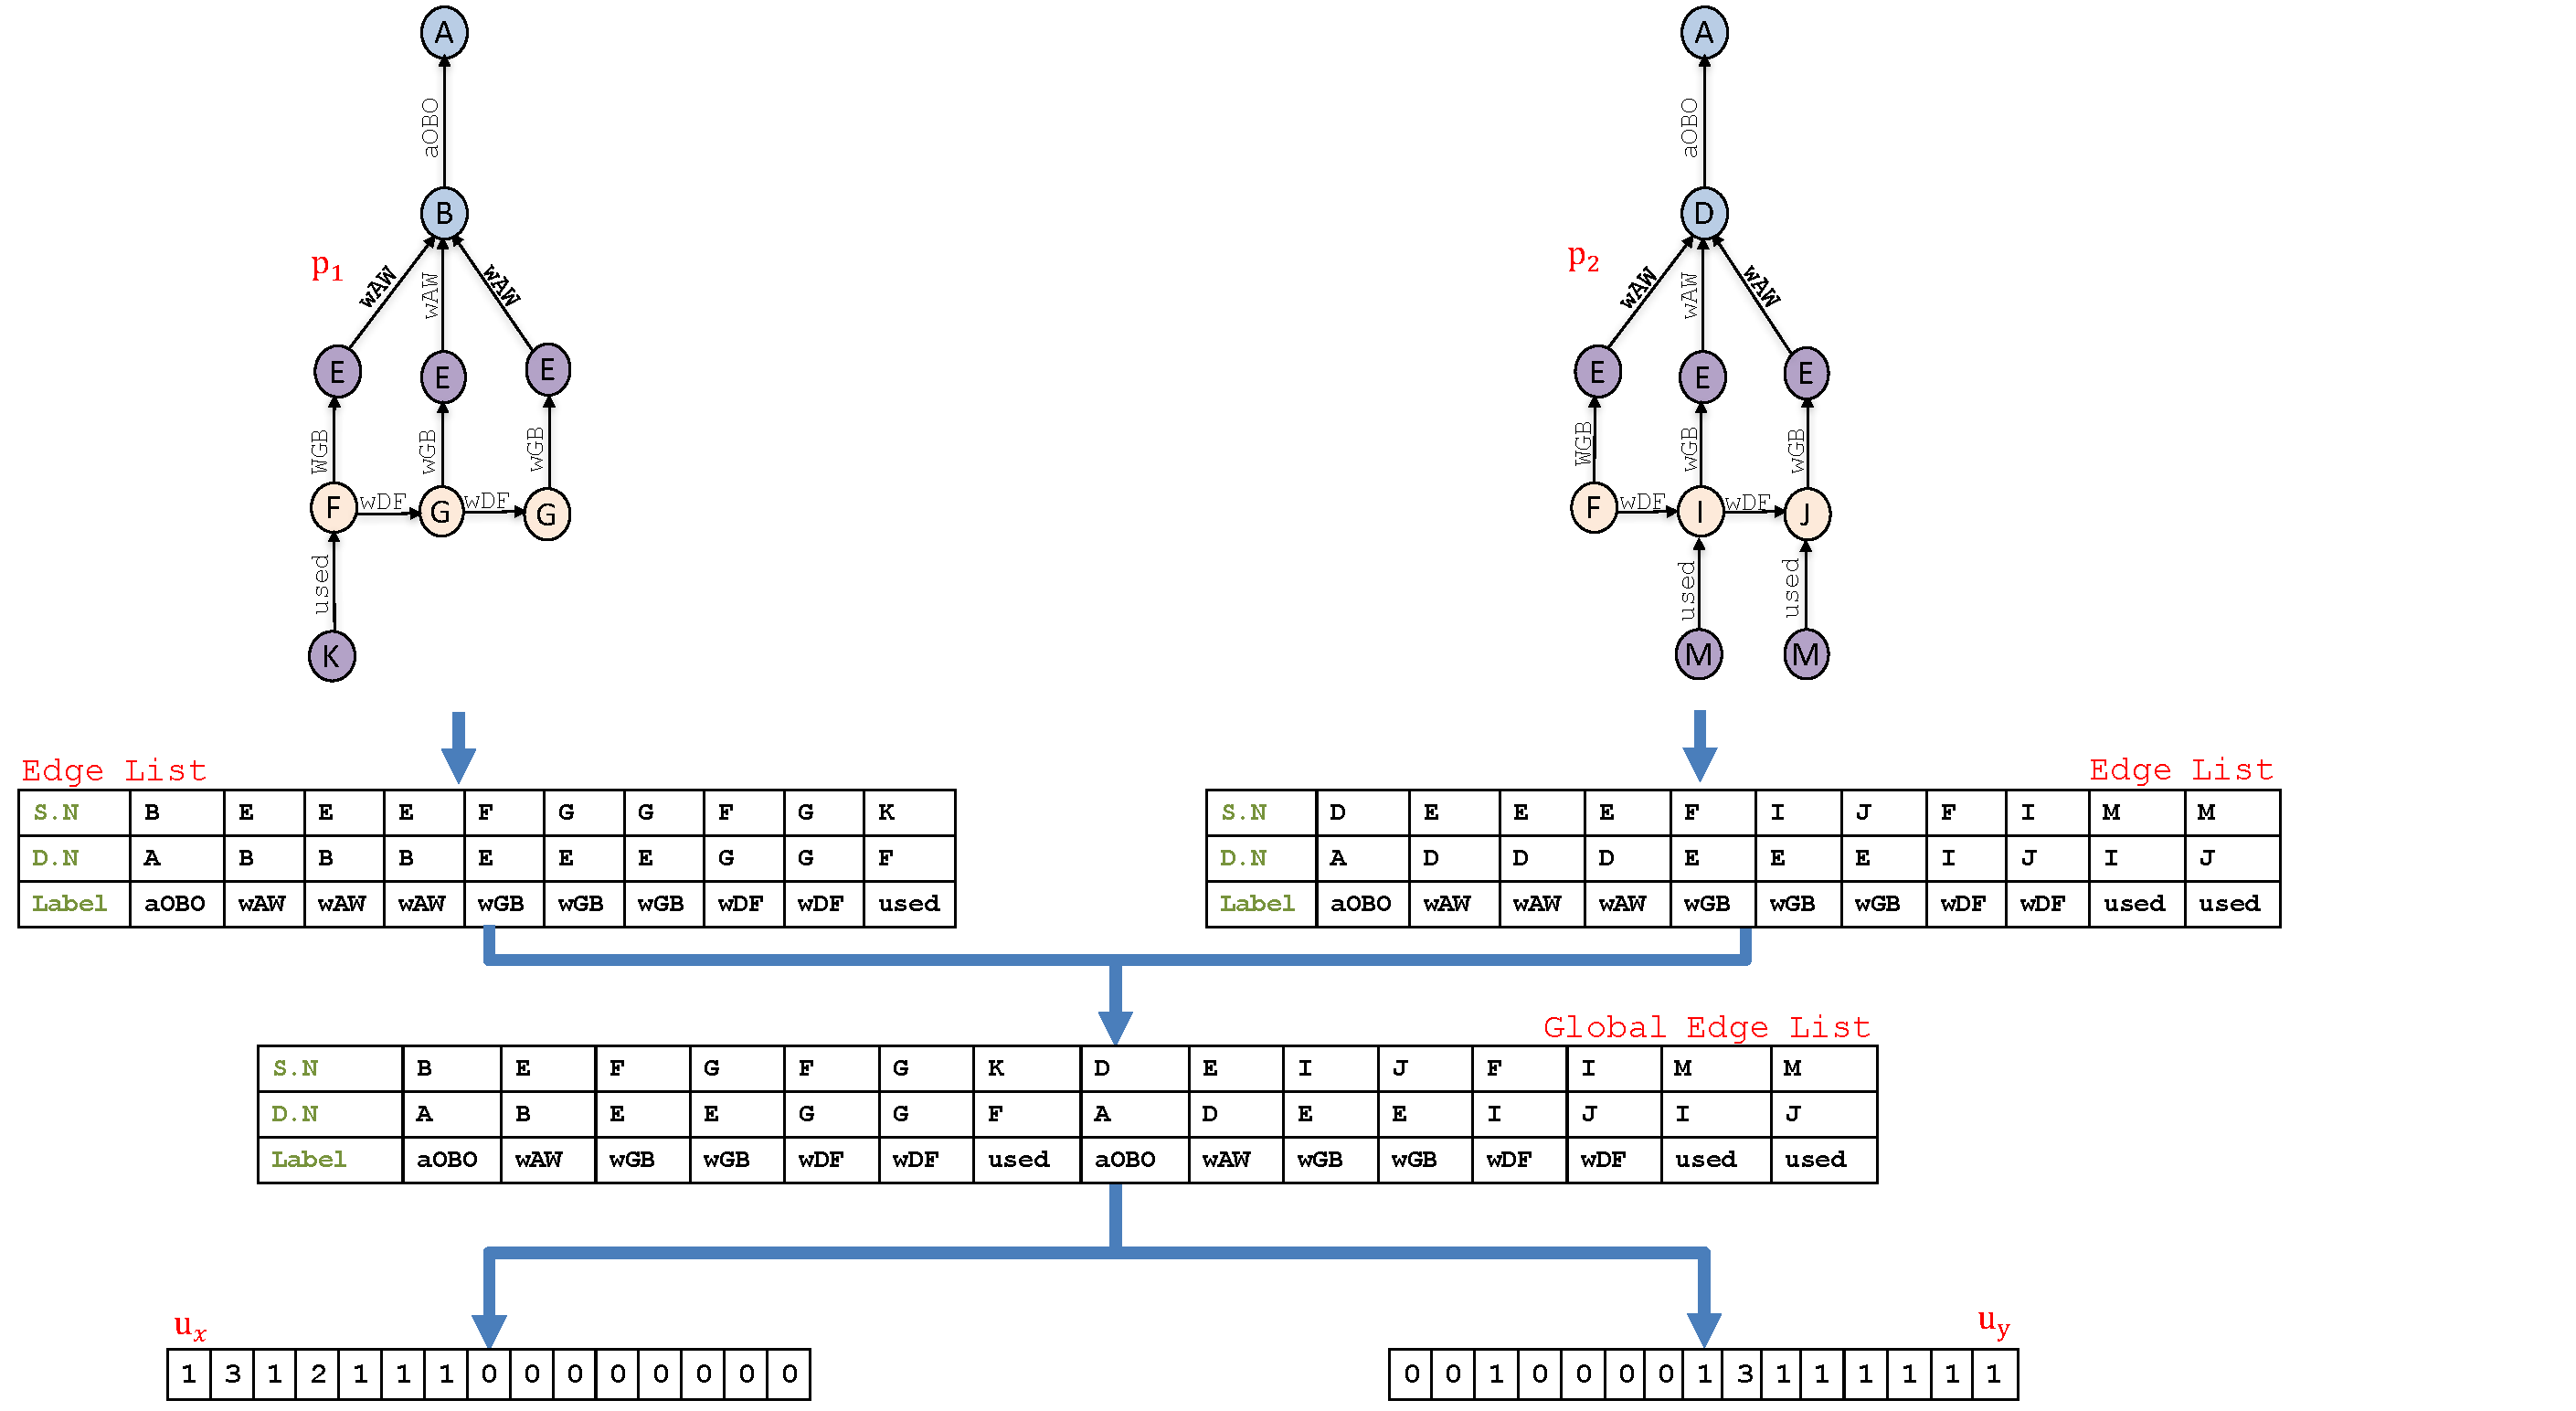
\includegraphics[width=\textwidth]{vector5.pdf}
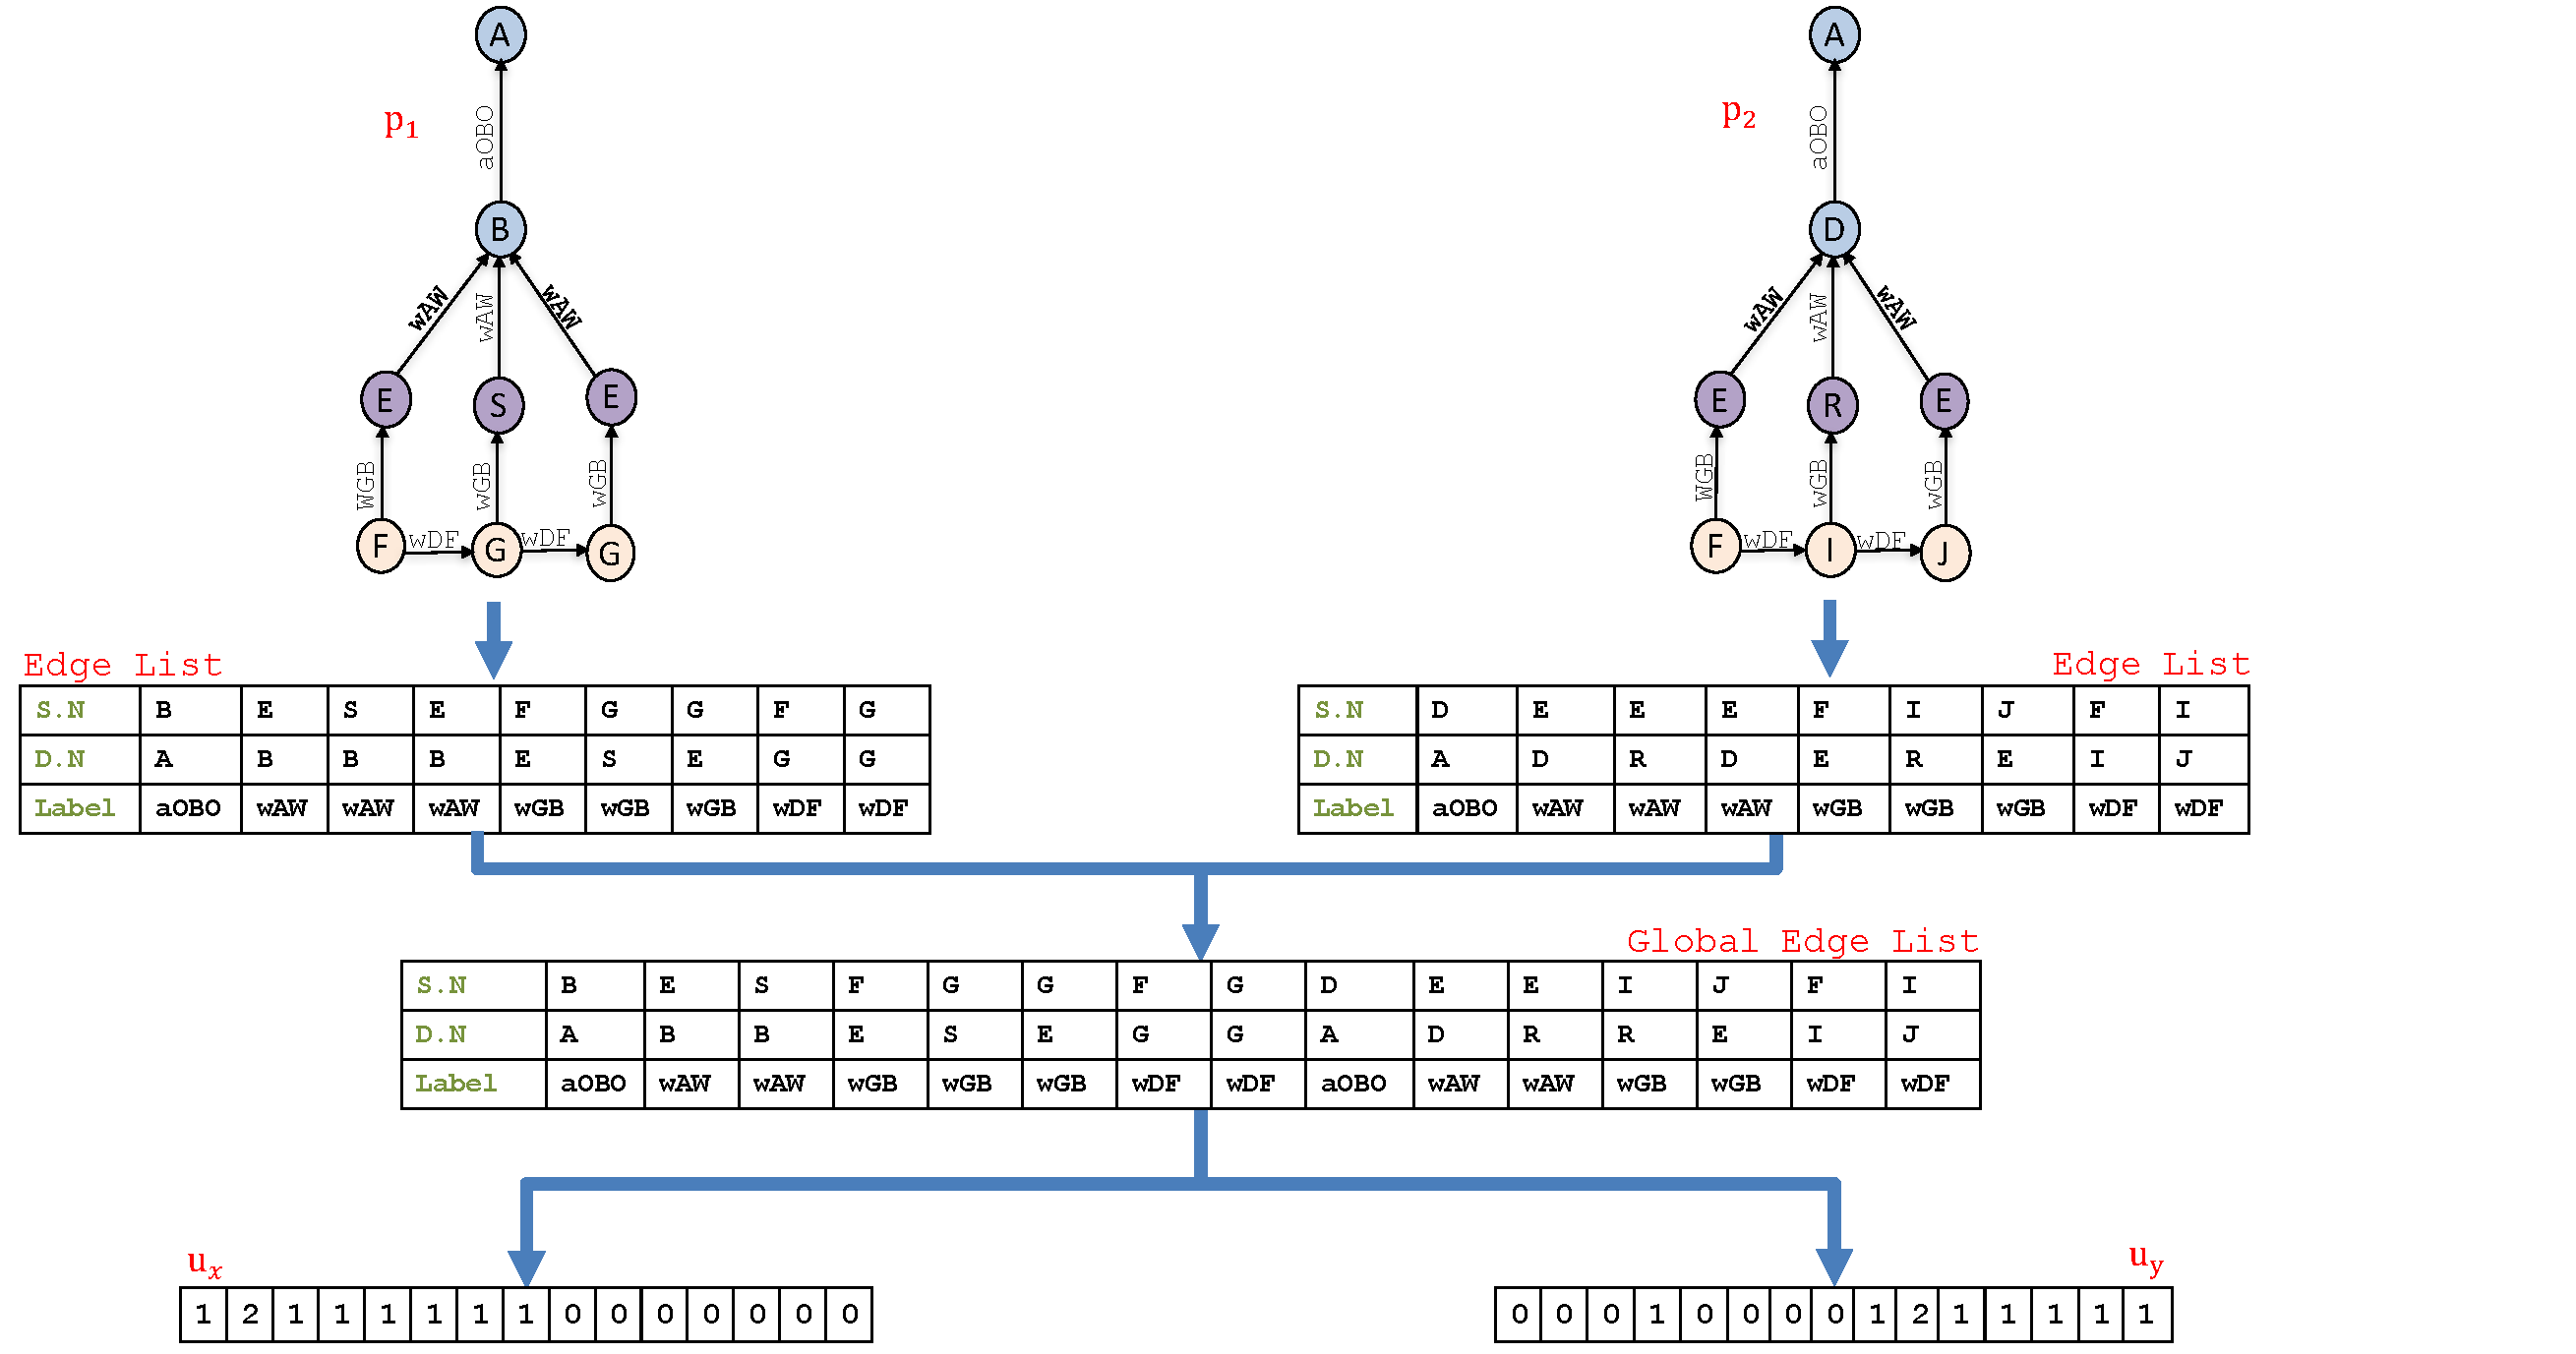
\includegraphics[width=\textwidth]{vector6.pdf}
\end{center}
\caption{Provenance graph conversion to vector space. $u_x, u_y$ represents the vectors generated from both provenance graphs}
\label{prov_vector}
\end{figure*}


\subsubsection{Defining an IoT application provenance graph}
%In an IoT application, there exist recurrent design patterns which can be leveraged to understand data flow. This information, can be leveraged to define the expected provenance graph for each application. 
Many IoT device consist of control systems in which sensor data is used as an input in a feedback loop to an actuator. The operations of most control systems are deterministic. This notion can be leveraged to define an expected provenance graph for each application. 


\par There are two types of control systems: open and closed loop control system. In an open loop control system, the system's output is not affected by the conditions (i.e. there are no feedback loop). An example of an open loop control system is a microwave. The timer is manually set to determine when the microwave stops regardless of the condition of its content (e.g. if the food is properly heated). However, in a closed loop control system, the system's output is used as feedback to influence the input.  An example of a closed loop system is a thermostat in which the temperature serves as output which is also used as an input feedback to regulate the temperature based on a predefined set-point. Using feedback as input increases the accuracy of an output. \par Each iteration of the control loop sequence generates a path in a provenance graph. The nodes contained along the path denote historical event transformations. For example, in a thermostat application, temperature readings generated might be converted from Celsius to Fahrenheit and utilized as feedback to an actuator or it could be stored locally or transmitted to a remote location. We focus on networked connected control system. Network connection opens doors to potential vulnerabilities





 


%Causality and dependency are concepts used to denote relationship between system events. Provenance graphs in turn be used in digital forensics \cite{zhang_outlier_2010} to investigate the cause of a malicious attack and also in intrusion detection systems to further enhance the security of computing devices. For further reading on provenance models and provenance graphs, we refer the reader to \cite{}  


 





%\subsection{Provenance-system collection}
%
%\subsubsection{Observed Provenance}
%
%\subsubsection{Disclosed Provenance}



%\subsection{Provenance Characteristics}
%
%Since provenance denotes the who, where and why of data transformation, it is imperative that data disseminated in an IoT architecture satisfies the required conditions. The characteristics of data provenance are outlined in detail below.
%
%
%\begin{itemize}
%
%\item Who: This characteristic provides information on activities made to an entity. Knowing the ``who" characteristic is essential because it maps the identity of modification to a particular data object. An example of ``who" in an IoT use case is a sensor device identifier.
%
%\item Where: This characteristic denotes location information in which data transformation was made. This provenance characteristic could be optional since not every data modification contains location details.
%
%\item When: This characteristic denotes the time information at which data transformation occurred. This is an essential provenance characteristic. Being able to tell the time of a data transformation allows for tracing data irregularities.
%
%\item What: This characteristic denotes the transformation is applied on a data object. A use case for IoT can be seen in the various operations (create, read, update, and delete) that could be performed on a file object.
%
%\end{itemize}
%
%
%There are two ways of pruning Provenance data: Provenance can be pruned at collection before it is been committed to the disk  or after being recorded to disk. Policy defines rules and actions that should be taken if any of the rules applies.  Access control in this case is used as a tool for pruning provenance data stored on an IoT device. It can also be extended for traditional access control measures. Data pruning is an essential problem for automatic provenance collection. Observed provenance and disclosed provenance. Observed provenance involves automatic collection of system states and changes. One major drawback of this method is that all system events are provenanced including irrelevant system provenance which incurs more storage overhead. Described provenance on the other hand, allows a user to provide a workflow of how what provenance the system is intended to generate and an engine to execute the workflow described.

%\subsection{ Document retrieval using vector space model} 
%Vector space conversion is used in information retrieval technique for determining document similarity to a query. Given a corpus $D = \{ d_1,..., d_n\}$, a query, $q$,  find document(s) ${d_x,....d_y}$ which are similar to $q$ and rank them by order of importance. To achieve this, documents are converted into a vector space representation which allows document to be ranked based on some similarity metric.
%
%
%\subsubsection{term frequency-inverse document frequency:}
%
%term frequency - inverse document frequency (tf-idf) is a widely used weighting scheme for ranking documents in a corpus given a query. The algorithm reflects how important a word is to a document. The more common a word is in a document, the higher the weighting factor. Given a term $t$ in document $d$ the term frequency $tf(t,d)$ is the number of times $t$ occurs in $d$.  tf-idf is composed of two algorithms: term frequency $tf$ and inverse document frequency, $idf$ .  tf-idf is derived from the product of tf and idf.
%
%  \[ tf-idf(t,d, D) = tf(t,d) \times idf(t,D) \]
%
%\par There are a number of ways to calculating the term frequency of a document. The first approach counts the raw frequency of each word contained in the document. 
% 
%
%\[ tf(t,d) = freq(t,d) \]
%
% 
% Another approach is to use boolean weighting. If a word is contained in a document, a weight of 1 is assigned as the term frequency, otherwise, a weight of 0 is assigned.
% 
% Other ways of computing the term frequency involves the use of the normalized instances of the term frequency. (i.e by dividing the frequency of each words by the total number of words contained in the document or by using the log of the raw frequency)
%
%  \[ tf(t,d) = \dfrac{freq(t,d)}{N} \]
%  
%   
% \[ tf(t,d) =  \log{(freq(t,d))} \]
% 
% 
%One major drawback of using the term frequency is that all terms in a document are considered equal while retrieving a query.In a corpus, some documents might contain words that are commonly repeated in every other documents. This adversely influences the weighting factor of a term in a corpus. For instance, in a collection of documents, words like  "the" are widely used and might occur more frequently.  Inverse document frequency (idf) ensures that frequently occurring words in a list of documents are given a lower weight than less occurring words. The more frequent a term occurs in a corpus, the less the idf weight.
%
% idf is computed by taking the log of the total number of documents in a corpus , $N$ divided by the number of documents which contains the term $df_t$.
% 
% \[idf(t, D) =\log \dfrac{N}{df_t} \]
% 
%tf-idf weighting scheme provides a vector space representation of documents. To compare the similarity between two documents, we employ the use of  a similarity measure such as cosine similarity, Jaccard similarity or euclidean distance. This similarity measures calculates some form of distance between the two vectors. Cosine similarity has been shown to outperform the rest of the similarity measures in comparing documents.

\subsection{Similarity Metric}
Similarity metric measures how identical two objects are. It compares the distance between data objects either by measuring the angle between the objects (cosine similarity) or a linear distance between the objects (euclidean distance). Similarity measures are widely used in document retrieval for selecting a query given a list of documents. 

\subsubsection{Cosine similarity}

This is a measure of orientation between the two non-zero vectors. It measures the cosine of the angle between the vectors. Two vectors which are at an angle of 90\degree  have a similarity of 0 while two vectors which are identical (with an angle of 0\degree) have a cosine of 1 and two vectors which are completely opposite (with an angle of 180\degree) have a similarity of -1. Since we are concerned with the similarity of the vectors, we are only concerned with the positive values bounded in [0,1]. To compute the cosine similarity between two vectors, $X$ and $Y$, cosine similarity is:

\[\mathbf{\cos{(\theta)}} = \dfrac{X \cdot  Y}{ \lVert \mathbf{X} \rVert \cdot \lVert \mathbf{Y} \rVert} =\dfrac{\sum_{i}^n X_i Y_i }{\sqrt[]{\sum_{i}^n X_i^2} \sqrt[]{\sum_{i}^n Y_i^2}}  \]

%\subsubsection{Jaccard Similarity}
%This similarity measure evaluates the intersection divided by the union of two non zero vectors.
%
%
%\[ J(X,Y) = \dfrac{|X \cap Y | }{| X \cup Y |} \]
%
%\subsubsection{Euclidean distance}
%This measures calculates the line distance between two data objects in an euclidean space. The euclidean distance between vectors $X$ and $Y$ , $d(X, Y)$ is defined by: 
%
%\[ d(X, Y) =  \sqrt{\sum_{i=1}^n (X_i - Y_i)^2} \]




%\subsection{A Review of Machine Learning Techniques: $DBSCAN$ and $k$-nearest neighbors}
%
%\subsubsection{$k$-Nearest Neighbors:} $k$-NN is an instance based supervised learning algorithm for data classification. Data is grouped on its similarity to nearest neighbors where $k$ denotes the number of neighbors in which the input data is compared to.  A similarity measure such as euclidean distance, jaccard similarity, or cosine similarity is used to measure the distance between vectors. $k$-NN can be applied to classification and regression problems.
%
%Researchers have proposed various modifications to the $k$-NN algorithm. Ramaswamy et al. \cite{Ramaswamy} proposed a $k$-NN modification which calculates the sparseness estimates for vectors in a dataset. The vectors are sorted in increasing order according the distance from its $k^{th}$ neighbor. Bay and Swabacher demonstrates how pruning irrelevant datapoint which are not considered anomalous can result in a linear complexity of nearest neighbor search for a randomized data. A threshold score is assigned which is based on the score of the weakest anomaly found. Pruning can be achieved by using the  relative density of data points, an anomaly is believed to occur in a group of data points with low density.
%
%\subsubsection{Density Based Spatial Clustering of Applications with Noise ($DBSCAN$):}
%
%\textit{DBSCAN} is a density-based clustering algorithm that differentiates regions with high density from regions with low density. It defines two parameters $\boldsymbol{\varepsilon}$, and $\boldsymbol{MinPts}$. $\varepsilon$ defines the maximum distance between two neighboring points in which they are considered to be in the same cluster. $MinPts$ is the minimum number of points that can be contained in a cluster. 
%
%Let $S = \{s_1, s_2,...s_n \}$ be a set of point to be clustered. $S$ consists of three point categories, a core point, $\boldsymbol{q}$, a border point, $b$ and a noise point, $n$. A core point is a point in which its $minPts$ are within distance $\varepsilon$. These are at the interior of the cluster. Border points are points on the edge of the cluster. A noise point (outlier) is any point that is neither a core point or a border point. A point, $l$ is directly reachable from a core point, $q$ if there exist a path which is within distance of $\varepsilon$ from the core another point. (i.e $ \exists \quad  \{q_1, q_2,...q_n \}, \textrm{where} \quad |q_{i+1}  - q_i| \leq \varepsilon$ ). A core point, $\boldsymbol{q}$ that is within distance $\varepsilon$ (i.e $q \leq \varepsilon$) is considered part of the same cluster. A border point is also considered part of a cluster if it close to a core point. A cluster consists of at least one core point.
%
%
%%\subsubsection{ $k$ means clustering:}







\section{Threat Model and Assumptions}
Due to the ubiquitous nature of IoT devices, there are a wide array of vulnerabilities associated with them. It is believed that each application exhibits a unique sequence of events which can be represented as the provenance graph of the application normal data flow. In designing our anomaly detection framework, we expect an attacker's footprint is reflected through the data flow as depicted in the provenance graph. Our algorithm detects attacks such as false data injection, modifications to the application code and the compromise to the integrity of data that exploits information flow of sensor events. 





%\section{Whitelist Approach}
%
%The whitelist approach consist of three phase: the data collection phase, the knowledge generation phase and the detection phase. The data collection phase involves generating provenance graphs. Provenance graphs are generated at normal program execution. The knowledge generation phase involves generating a repository of provenance graphs of  various IoT applications with normal executions, free from malicious activities. The knowledge  repository contains an exhaustive list of known provenance graphs for various IoT applications. Each, IoT Application exhibits a unique data flow path which is represented in their provenance graph. The knowledge repository is updated by knowledge experts pertaining to the IoT application. Finally, in the detection phase, the application's provenance graph being observed is compared to the provenance graph contained in the knowledge repository. If there is a direct match, the running application is considered to be running as expected, otherwise an alert such as a warning is generated and the application is flagged for possible intrusion. 

%\begin{figure}[h!]
%\begin{center}
%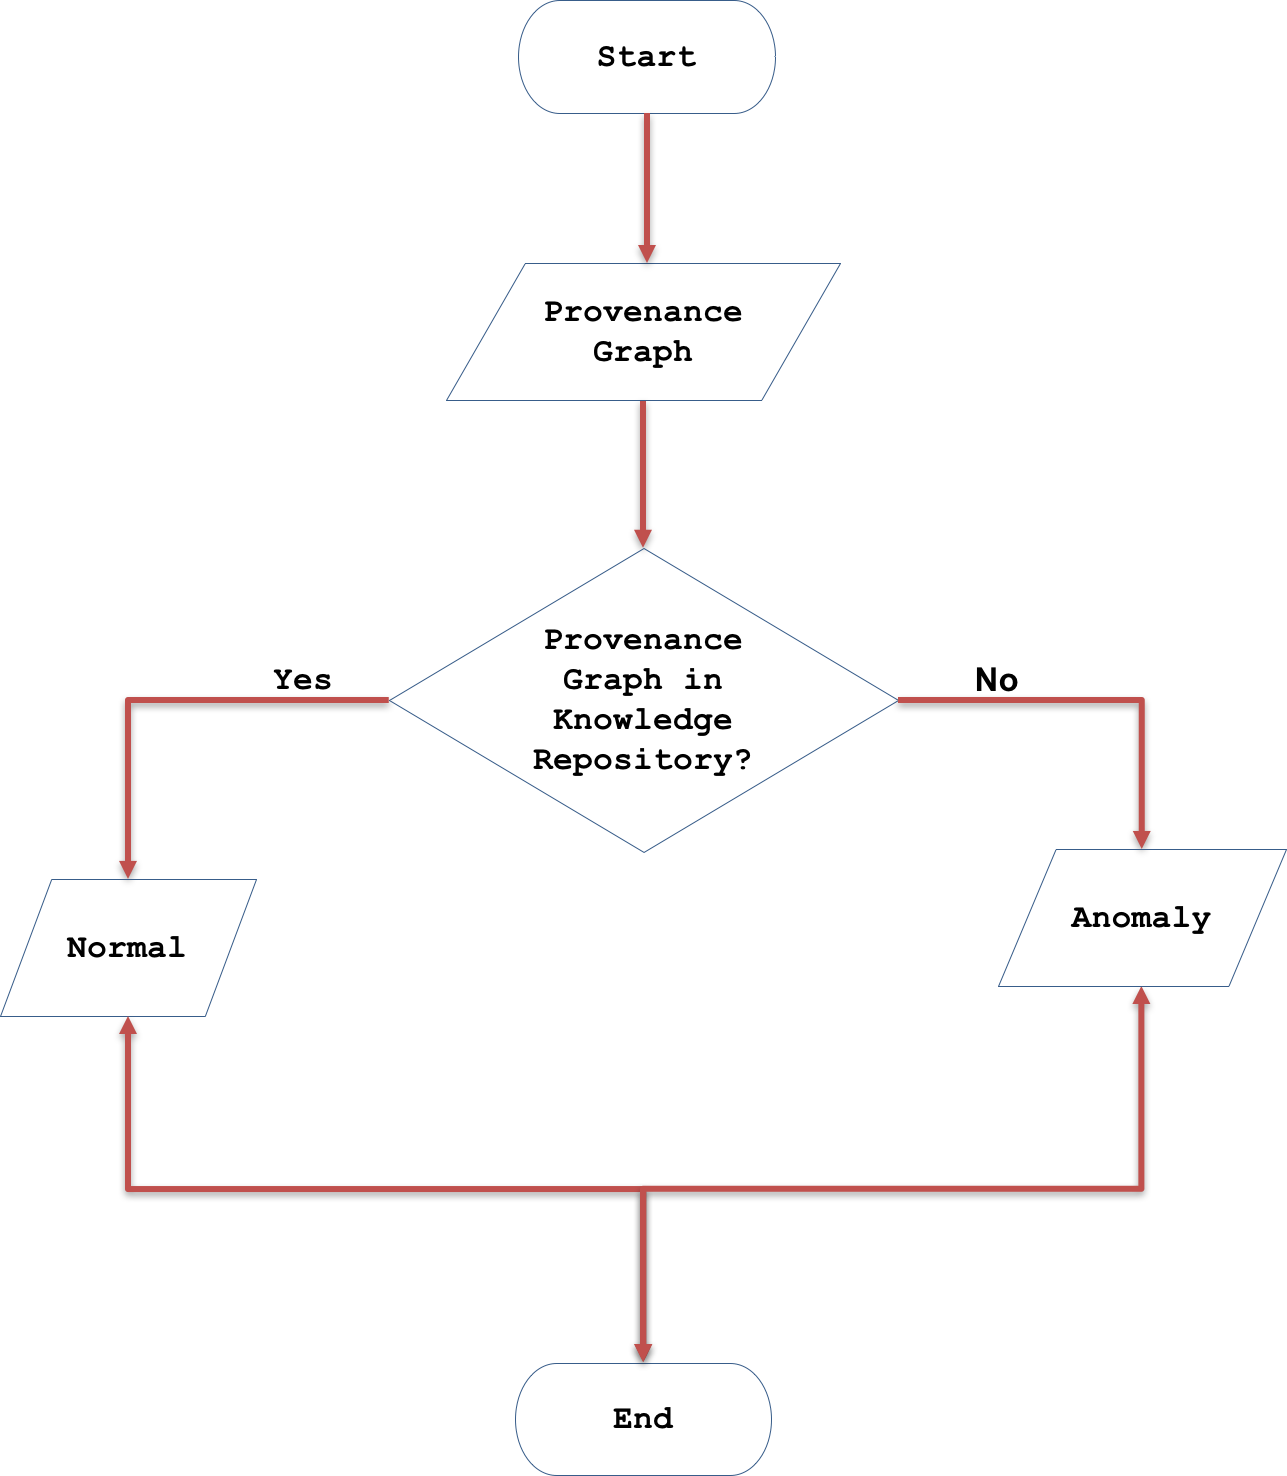
\includegraphics[height=4in, width=3.5in]{whitelist.png}
%\end{center}
%\caption{Whitelist approach to anomaly detection}
%\label{whitelist}
%\end{figure}


\section{Graph Similarity Anomaly Detection}

The expected regularity of provenance graphs in IoT applications motivate a graph-based approach to anomaly detection. This approach consists of two phase: observation phase, also known as the training phase and the test or detection phase. In the observation phase, the system collects provenance data considered to be a representation of the normal system behavior. In the detection phase,  provenance graph from the observation phase is compared with the provenance graph derived from subsequent observations to determine if an anomaly exists. 


\subsection{Provenance Graph to Vector Space Conversion }

Our method of comparing the similarity of provenance graphs was inspired by an information retrieval technique for document retrieval. Given a corpus $D = \{ d_1,..., d_n\}$, and query, $q$, how do we find document(s) $\{d_x,....d_y\}$ which are similar to $q$ and rank them by order of importance. To achieve this, documents contained in the corpus are converted into a vector space representation which allows documents to be ranked based on some similarity metric. 


%\begin{figure}[h!]
%\begin{center}
%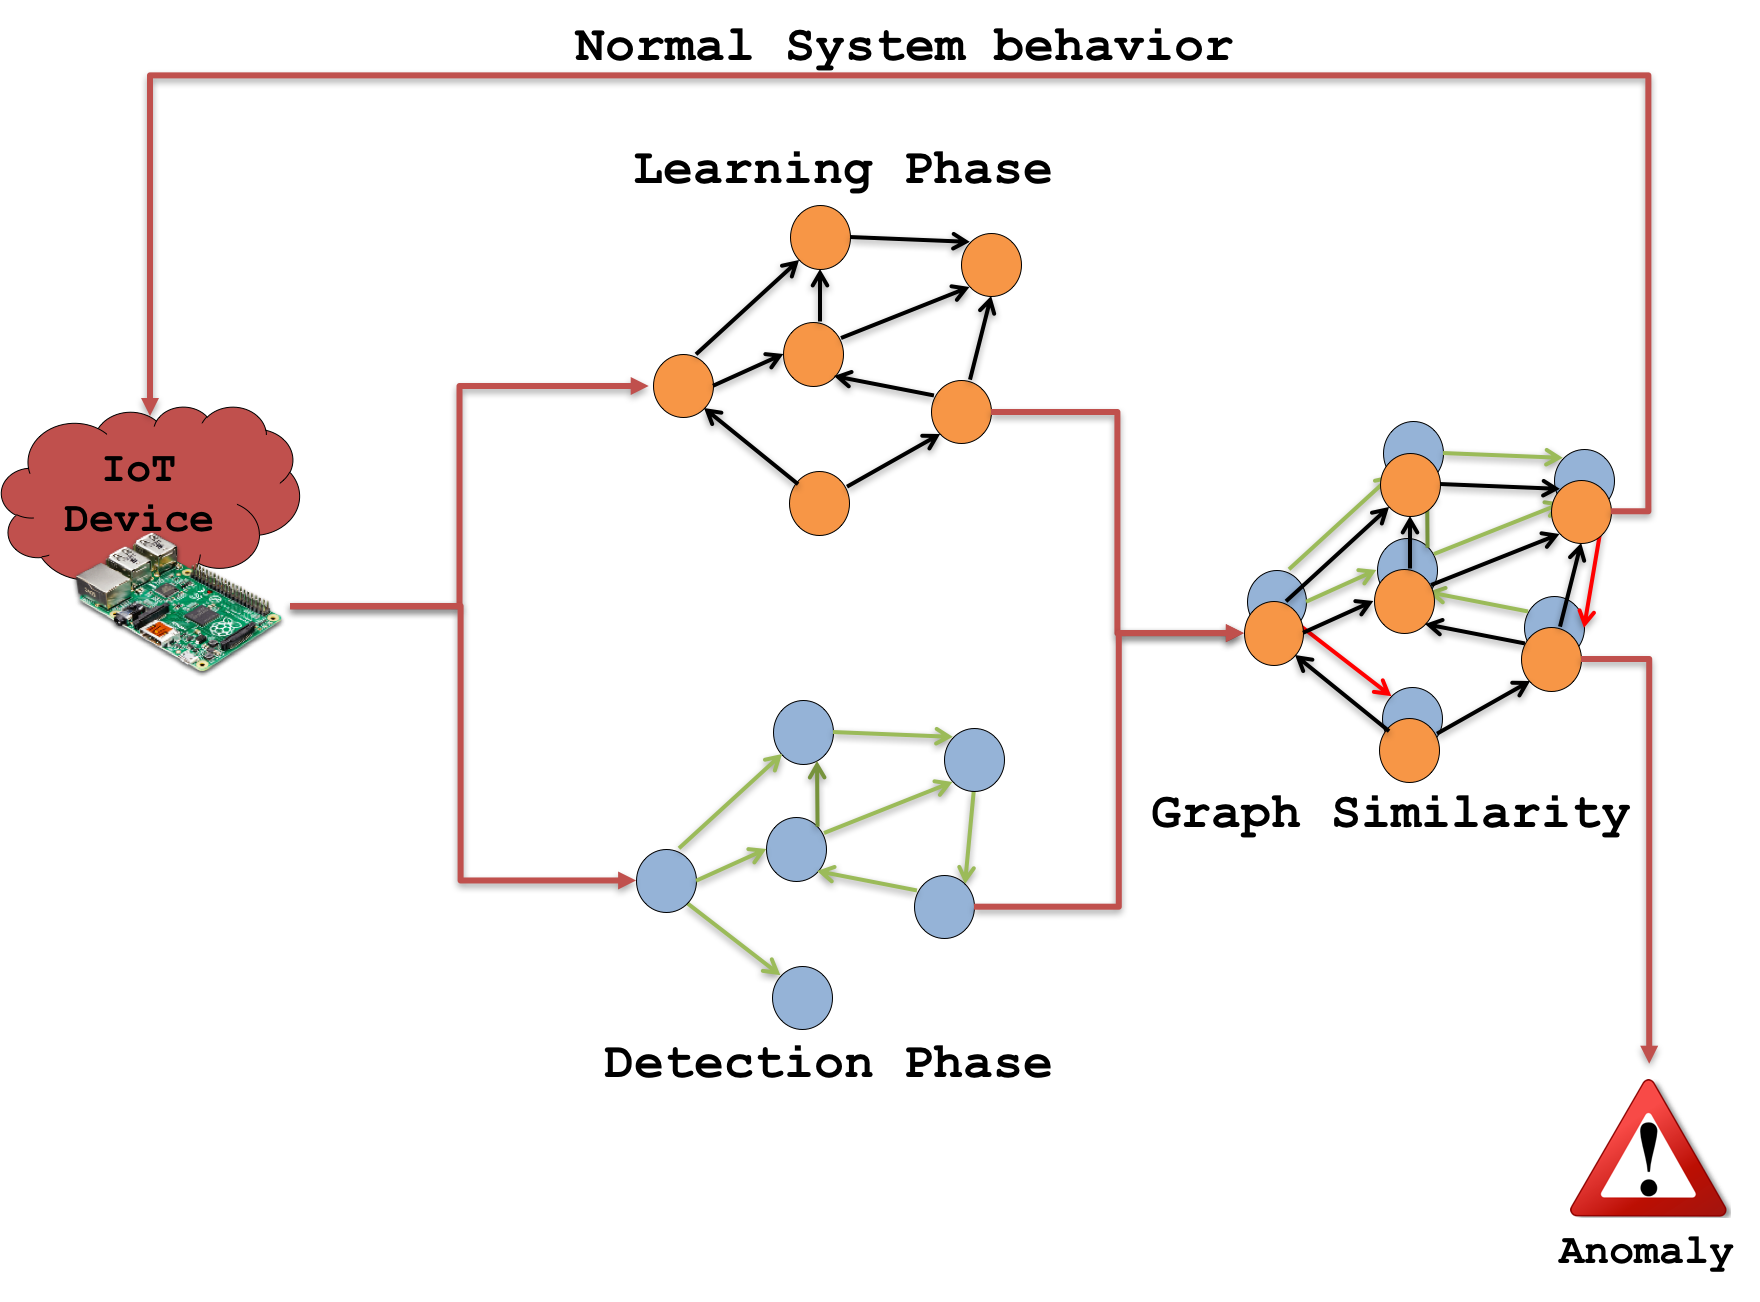
\includegraphics[height=2.5in, width=3.5in]{similarity_5.png}
%\end{center}
%\caption{Graph Similarity Approach}
%\label{graph_similarity}
%\end{figure}



\subsubsection{Provenance Graph Feature Extraction}

A similarity function measures how identical two provenance graphs are in a vector space. In order to apply a similarity function, we compute a vector representation. In this approach, a provenance graph undergoes dimensionality reduction into an $n$-dimensional vector space where $n$ represents the number of unique edges (global set of edges) contained in the provenance graph set. This representation is used as input to our anomaly detection algorithm. \par Selecting the most appropriate feature from provenance graphs is an important task. We need to utilize features that preserves the order of edges and nodes contained in the provenance graph. Our approach utilizes the occurrence of unique edges contained in both graphs.  
%\par We provide a means of classifying such edges as identical. To determine identical edges, we utilize a combination of edge labels and source and destination node. That is, for two edges to be considered identical, they must contain identical labels and contain identical source and destination nodes. We say two edges $E_x $ and $E_y$ are identical (denoted $E_x \sim E_y$) if $E_x.V_s = E_y.V_s$, $E_x.V_d = E_y.V_d$, and $E_x.label = E_y.label$  

\par We provide a means of classifying such edges as identical. To determine identical edges, we utilize a combination of edge labels and source and destination node.That is, two edges $e_x $ and $e_y$ are identical (denoted $e_x \sim e_y$) if $e_x.v_s = e_y.v_s$, $e_x.v_d = e_y.v_d$, and $e_x.label = e_y.label$  

%\par In performing our graph to vector space conversion, we define a set of procedures. First, we define our edge identification function as follows: 


%\begin{definition}
%
%%Consider a provenance graph, $p = (V, E)$ where $E = \{E_i,...E_n\}$ and $E_i = (n_s, n_d, label)$. $n_s, n_d$ are source and destination vertices respectively $ \mid n_s, n_d \in V$.  The equivalency function of two edges $eq(E_x, E_y)$  is $ E_x = E_y  if E_x \rightarrow n_s  \&  E_y \rightarrow n_s $  
%
%%Consider a provenance graph, $p = (V, E)$ where $E = \{E_0,...E_n\}$ and $E_i = (n_s, n_d, label)$. $n_s, n_d$ are source and destination nodes respectively such that $ n_s, n_d \in V$. Edges $E_x $ and $E_y$ are considered identical if $E_x.n_s = E_y.n_s$ and $E_x.label = E_y.label$  
%
%
%Consider a provenance graph, $p = (V, E)$ where $E = \{E_1,...E_n\}$ and $E_i = (V_s, V_d, label)$. $V_s, V_d$ are source and destination vertices respectively such that $ V_s, V_d \in V$. The edge identification function $\delta$ is defined as:  $E_x $ and $E_y$ are considered identical (i.e. $E_x \sim E_y$) iff $E_x.V_s = E_y.V_s$, $E_x.V_d = E_y.V_d$, and $E_x.label = E_y.label$  
%
%\end{definition}
 





%Edges contained in a provenance graph yet distinct could posses identical edge labels that can be utilized. 





%\begin{figure}[h]
%\begin{center}
%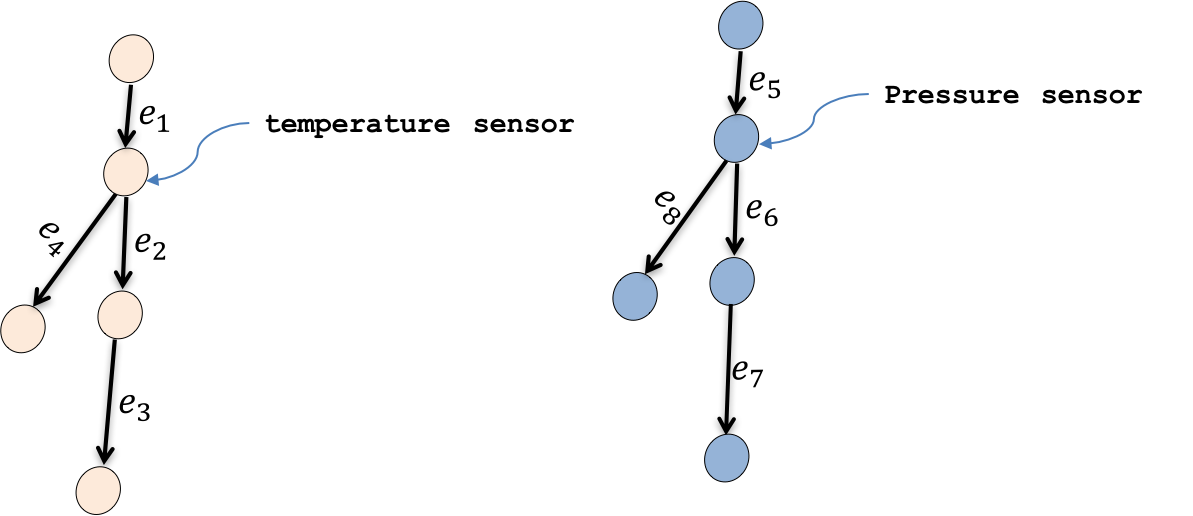
\includegraphics[height=1.7in, width=3.5in]{sensor_vector.png}
%\end{center}
%\caption{Edge identification between two graphs. Identical events from Different sensor nodes corresponds to different edges}
%\label{example}
%\end{figure}



An edge list $E_{p}$ consists of all of the edges contained in $p$. A global edge list $E_{G}$ consists of all non-similar edges contained in $P$. $E_{G}$ preserves the ordering of edges contained in $P$ in the vector space. 
%since all generated vectors are derived from its ordering.

\begin{definition}

Let $P = \{p_1,...,p_n\}$ such that $p_i = (V, E)$. $E_{G} = \{ e_1,...,e_n\} \mid E_{G}  \in P$ where $e_i \neq e_{i+1}, 1 \leq i \leq n$. $E_{p} \gets \{e_1,...,e_n\} \mid E_{p} \in p$ where  $e_{pi} \neq e_{pi+1}, 1 \leq i \leq n$

\end{definition}


Finally, we define our provenance graph to vector approach as follows:

\begin{definition}
Let $P = \{p_1,...,p_n\}$ where $p_i = (V, E)$. The vector space representation of $p_i, \boldsymbol{u_i}$, is the number of times edges contained in $E_{p}$ occurs in $E_{G}$. $\boldsymbol{u_i}$ has a length of $k$ which consists of all of the unique edges contained in the global edge list  $E_{G}$. 


%Unique edges are found by identifying similar edges and a frequency count of the number of edges. 


 
%
%\[ \boldsymbol{v_x} = ( freq(E_i, p_i)) \]
%
%where $freq$ denotes the occurrence of $E_i$ in graph $p_i$

\end{definition}



Figure \ref{prov_vector} displays the vector space conversion of provenance graphs. $\boldsymbol{p_1}$, and $\boldsymbol{p_2}$ consists of vertices $A,B,E,F,G, I, J, K, M$ and edges $aOBO, wAW, wGB, wDF$. The vector representation of graphs, $u_1$, and $u_2$ is the occurrence of edges contained in the edge list that is found in the global edge list. 

%\[ \boldsymbol{v_1} = (2,1,1,1,1) \] \[\boldsymbol{v_2} = (1,2,0,1,1,1,0) \]

%\begin{figure}[h]
%\begin{center}
%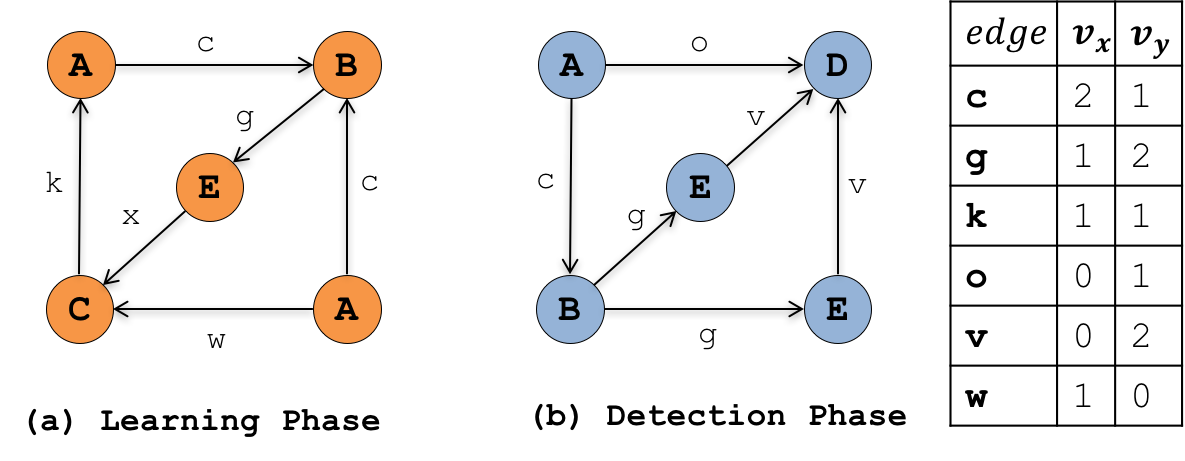
\includegraphics[height=1.7in, width=3.5in]{graph_sim_update.png}
%\end{center}
%\caption{Provenance graphs and their vector representation. $v_x, v_y$ represents the vectors generated from the learning and detection phase respectively}
%\label{example}
%\end{figure}



%\begin{multicols}{2}
%\lipsum[1-7]
%\end{multicols}




\subsection{Graph Based Similarity Detection Algorithm}

Given $u_x, u_y$ which denotes the vector representation of provenance graphs $p_x, p_y$. The similarity of $p_x, p_y$ is found by calculating the cosine similarity between the two vectors where 1 denotes similarity between the two vectors and 0 denotes non-similarity between the two vectors. A threshold value is set which is used to classify the behavior of provenance graphs in the detection phase as normal or an anomaly.

\[sim(u_x,u_y) =  \dfrac{u_x \cdot  u_y}{ \lVert \mathbf{u_x} \rVert \cdot \lVert \mathbf{u_y} \rVert} =\dfrac{\sum_{i=1}^n u_{xi} u_{yi} }{\sqrt[]{\sum_{i=1}^n u_{xi}^2} \sqrt[]{\sum_{i=1}^n u_{yi}^2}}  \in [0,1] \]


Algorithm 1 depicts a formal definition of the graph-based similarity algorithm.




\begin{figure}[h!]

\begin{algorithmic}[1]



% \SetKwInOut{Input}{Input}
% \SetKwInOut{Output}{Output}


\Procedure{GraphSetToEdgeList}{$P$}
%\Input{Two nonnegative integers $a$ and $b$}
%\State $p_i\gets (V, E)$
%\State $E_i = (V_s, V_d, label)$

%\State $E_P \gets \{E_0,...,E_n\} \mid E_P \in P$ where  $E_{Pi} \neq E_{i+1}, 0 \leq i \geq n$   
%\State $E_p \gets \{E_0,...,E_n\} \mid E_p \in p$ where  $E_{pi} \neq E_{i+1}, 0 \leq i \geq n$   


%\State $V = \{V_0,...V_n\}$


%\State $[v_x, v_y] \gets DistinctEdgeFreq(G_x, G_y)$   


%\For{$p_i \in P$}

\State \textbf{INPUT: } $P=\{p_0,...,p_n\} \mid p_i\gets (V_i, E_i), 0 \leq i < n.$

\State $E_G \gets \{\}$

\For{$p_i = (V_i, E_i) \in P, 0 \leq i < n$}

\For{$e_j \in E_i$}

\If{$e_j \not\in E_G$}
\State $E_G = E_G \cup e_j$
\EndIf

\EndFor

\EndFor
\State \textbf{return} $E_G$

\EndProcedure
\end{algorithmic}


\begin{algorithmic}[1]
\Procedure{GraphtoVector}{$p \gets (V,E), E_G$}

\State $k = |E_G|$

\State $Q[k] \mid Q[i] \gets 0, 0 \leq i < k$


\For{$e_j \in E$}

%\State \textit{Found} $\gets$ \textbf{False}

\For{$e_g \in E_G \mid 0 \leq g < k$}

\If{$e_j \sim e_g$}
\State $Q[g] \gets Q[g] + 1$
%\State \textit{Found} $\gets$ \textbf{True}
\EndIf

\EndFor

\EndFor


\State \textbf{return} $Q$

\EndProcedure
\end{algorithmic}

\begin{algorithmic}[1]

\Procedure{GraphAnomaly}{$P,p$}

\State $E_G \gets GraphSetToEdgeList(P \cup p)$

\State $Q \gets GraphtoVector(p, E_G)$ 

\For{$p_i \in P$}
\State $N_i \gets GraphtoVector(p_i, E_G)$

\State $z \gets sim(Q, N_i)$
\If{z $\geq$ threshold}
\State \textbf{return} normal

\EndIf

\EndFor	

\State \textbf{return} anomaly
\EndProcedure



\end{algorithmic}


\caption{Graph based anomaly detection algorithm}\label{alg:graph_anomaly}
\end{figure}


%\subsubsection{Algorithm}




\subsubsection{Defining Anomaly Threshold}

An anomaly threshold $t$ is a score that defines at what point a provenance graph contained in the test data is considered anomalous. Ensuring a proper threshold score is used for detection is an important task that requires extensive knowledge of the application domain. The threshold is manually set to a value $t$, which is defined by domain experts. For automatic anomaly threshold detection, one can use prediction methods to define the anomaly score. Prediction techniques are beyond the scope of this paper. 

%\subsubsection{Computational Complexity:}
%
%\textcolor{red}{  TODO}






\section{Experiment}

This section outlines experimental procedures involved in evaluating our proposed algorithm. 


\subsection{Experimental Setup}

We evaluate our intrusion detection algorithm by implementing an IoT application which simulates a climate control system. Constant irregularities in temperature could have devastating effects on industrial machinery. Climate control systems ensures a proper functional environment for people and machinery. This system consist primarily of a Heating Ventilating and Air Conditioning (HVAC) System which uses temperature, humidity data to regulate environmental conditions within a building. The temperature is set within a bounded limit such that when the temperature exceeds a certain threshold, a cooling phase is activated and the air conditioning is switched on until the temperature decreases below a threshold in which the heating phase is activated in which the heater is turned on.

\par In order to evaluate the effectiveness of our proposed approach, experimental  evaluation was performed on Raspberry Pi 3 with 1 GB of memory running Ubuntu mate. For our implementation of our simulated climate control system, we utilized a publicly available dataset \cite{LANGEVIN201594} which consists of a year's worth of longitudinal data on the thermal conditions, related behaviors, and comfort of twenty-four occupants in a medium-sized building. This dataset consist of temperature, humidity, air velocity, and voltage readings at varied date and time intervals, collected from a total of 24 sensors with a duration of fifteen minutes. We utilize the temperature and humidity data as input to our aforementioned simulation program.




% To build our knowledge repository, we ran our IoT application executing in a normal environment and the resultant provenance graph produced was stored in Neo4j, a graph database for efficient graph processing. To generate our malicious attack dataset, we simulate a false data injection attack by introducing constant and irregular temperature and values to our original dataset.


\subsection{Preliminary Experimental Result}

To build our knowledge repository, we generate provenance graphs for each week contained in a year. We compare the provenance graph generated for various weeks to see how they differ using our graph similarity approach.


%We evaluate the performance of our proposed algorithms by calculating three performance metrics: false positive, true positive and false negative rate. False positive indicates when an intrusion that does not exist is detected, false negative indicates when the IDS classifies a provenance graph as normal when it is malicious, finally for true positive an IDS classifies a provenance graph as anomalous which is actually an intrusion.  Detection rate, false alarm rate and false negative rate are calculated as follows: 
%
%  \[Detection\, rate =  \dfrac{TP }{TP + FN}\] 
%  \[False\, alarm\, rate =   \dfrac{FP }{FP + TN}\] 
%  \[False\, negative\, rate =  \dfrac{FN }{FN + TP} \]


%Provenance graphs were generated using an IoT applications running on the raspberry pi 3. The first application simulates a Heating Ventilation, AC system and the other application simulates a. To generate malicious attack dataset, we utilized simulated data of how provenance graphs will look in an event of an attack. This graph was generated and agreed on by domain experts. To build our knowledge repository, we ran our IoT applications and the resultant provenance graph is stored in Neo4j, a graph database for efficient graph processing.


%\subsection{Discussion}
%
%\textcolor{red}{TODO}




\section{Related Work}

There has been a considerable amount of research done on anomaly detection. Most of the work involves the analysis of system call sequence. Liao et al \cite{liao_using_2002} characterizes a system's normal behavior by denoting the frequency of unique system calls which are converted into a vector space representation. A classification algorithm such as $k$-Nearest Neighbors is used to classify the training data set. Stephanie et al \cite{Hofmeyr} defines a link between the human immune system and intrusion detection systems. They develop a normal system behavior repository by analyzing system call sequences of an application. The application's system call sequence is stored in a normal database which is queried during observation where all behaviors are judged. If an application executes a sequence of system calls that are not found in the normal database, a mismatch is recorded. If the mismatch for that application exceeds a threshold, an anomaly is detected. Yoon et al. \cite{Yoon} developed a technique for intrusion detection on embedded systems by analyzing system call frequencies. This is achieved by learning normal system profile of observed patterns in the system call frequency distribution.Their hypothesis is that applications follow a known frequency pattern which is centered around the centroid. Data from the training set is  clustered using k-means which groups legitimate system behavior. Observation at run-time are compared with the clusters in the detection phase, if the incoming observation does not fit into a cluster, it is considered an anomaly. \par Additionally, anomaly detection on graphs has also been explored. Manzoor et al \cite{manzoor_fast_2016} proposed a centroid based clustering anomaly detection for instances of streaming heterogeneous graphs in real time.  This algorithm is able to accommodate incoming edges in real time. 
%They propose a method of comparing the similarity between heterogeneous graphs by comparing the similarity of two graphs by their relative frequency. Each graphs is represented as a vector known as shingles. Since all of the graph is stored in memory, they also accommodate an efficient representation of the shingles in memory in what is known as streamhash. 
Papadimitriou et al \cite{Papadimitriou2010} proposed five similarity algorithms for comparing the similarity of web graphs namely signature similarity, vertex/edge vector similarity, vertex ranking,and vertex edge overlap. These algorithm are inspired by document similarity method namely shingling and random projection based method. Nodes represents a webpage and  an anomaly could indicate a missing link (edge) or a web node. Out of the five similarity measures proposed, signature similarity which compares two graphs based on a set of features (signatures) using a scheme known as \textit{simHash} performed the best followed by vector similarity. By comparing instances between snapshot of crawled webpages, this enables the detection of inconsistencies in crawled web content. Noble et al \cite{Noble} proposed two algorithms for anomaly detection in graphs The first approach, looks at unusual substructures in graphs. This is achieved by inverting the subdue score of patterns that occurs frequently in a graph. Subdue is a method for detecting substructures within graphs. The values that produce high scores are flagged as anomalies. The second approach examines unusual subgraphs contained in a graph by iteratively using subdue algorithm to compress the graph. The idea behind this method is that subgraphs containing many common substructures are considered less anomalous than one with less substructures. Some graph approach involve the use of a community-based approach in which dense regions of connected nodes are considered normal and nodes with high sparse regions which do not belong to any community are considered anomalous. \textit{AUTOPART} \cite{chakrabarti2004autopart} consist of nodes with similar neighbors are clustered together and the edges which do not belong to any cluster are considered as an anomaly. To detect communities, it achieves this task by reorganizing the rows and the columns of the adjacency list.

% Our approach of graphs similarity is similar to graph kernels and graph edit distance. graph kernels involves measuring the similarity between two graphs, graph edit distance looks at the number of operations required for a graph $G_1$ to be identical to $G_2$. 


\section{Summary and Conclusion}

In this paper, we propose an anomaly detection algorithm for detecting anomalous instances of sensor based events in an IoT device using provenance graphs. We implemented and evaluated the functionality of our approach on an IoT application which simulates a climate control system.  Our preliminary results feasible and show promise. We plan on conducting further detailed experiments to identify false positives, true positives, and false negative rates. We also plan on investigating the application of our approach in the automotive domain by understanding how provenance graphs can be used for anomaly detection in vehicular network intrusion.




\section{Acknowledgment}
This research has been supported in part by US National Science Foundation (CNS grant No. 1646317). Any opinions, findings and conclusions or recommendations expressed in this material are those of the author(s) and do not necessarily reflect the views of NSF.






% For peer review papers, you can put extra information on the cover
% page as needed:
% \ifCLASSOPTIONpeerreview
% \begin{center} \bfseries EDICS Category: 3-BBND \end{center}
% \fi
%
% For peerreview papers, this IEEEtran command inserts a page break and
% creates the second title. It will be ignored for other modes.
\IEEEpeerreviewmaketitle









% trigger a \newpage just before the given reference
% number - used to balance the columns on the last page
% adjust value as needed - may need to be readjusted if
% the document is modified later
%\IEEEtriggeratref{8}
% The "triggered" command can be changed if desired:
%\IEEEtriggercmd{\enlargethispage{-5in}}

% references section

% can use a bibliography generated by BibTeX as a .bbl file
% BibTeX documentation can be easily obtained at:
% http://mirror.ctan.org/biblio/bibtex/contrib/doc/
% The IEEEtran BibTeX style support page is at:
% http://www.michaelshell.org/tex/ieeetran/bibtex/
%\bibliographystyle{plain}
% argument is your BibTeX string definitions and bibliography database(s)
%\bibliography{refrences}
%
% <OR> manually copy in the resultant .bbl file
% set second argument of \begin to the number of references
% (used to reserve space for the reference number labels box)

%\begin{thebibliography}{1}
%
%\bibitem{IEEEhowto}
%H.~Kopka and P.~W. Daly, \emph{A Guide to \LaTeX}, 3rd~ed.\hskip 1em plus
%  0.5em minus 0.4em\relax Harlow, England: Addison-Wesley, 1999.
%
%\end{thebibliography}


\bibliographystyle{IEEEtran}
\bibliography{bibliography}


% that's all folks
\end{document}


